\documentclass[12pt,twoside]{report}
\usepackage[utf8]{inputenc}
\usepackage{datetime}
\usepackage[a4paper,width=150mm,top=25mm,bottom=25mm,bindingoffset=6mm]{geometry}
\setlength{\headheight}{15pt}

% fancyhdr
\usepackage{fancyhdr}
\newcommand{\changefont}{%
    \fontsize{9}{11}\selectfont
}
\pagestyle{fancy}
\fancyhead[LE,RO]{\changefont \slshape \rightmark} %section
\fancyhead[RE,LO]{\changefont \slshape \leftmark} %chapter

% graphicx
\usepackage{graphicx}
\graphicspath{{images/}}

% biblatex
\usepackage[square,numbers]{natbib}
\bibliographystyle{unsrtnat}

\usepackage[nottoc]{tocbibind}

\title{
    {Agent-based Strategies in Maze-like Environments}\\
    {\large Babeș-Bolyai University}\\
    {
        \begin{figure}[h]
            
\includegraphics[width=5cm]{logo_cs.png}
            \centering
        \end{figure}
    }
}
\author{Mihnea Ungureanu}
\date{June 2020}

\begin{document}

\maketitle

\chapter*{Abstract}
Over the relatively recent years, \textbf{reinforcement learning (RL)} has gained immense popularity.
Stemming from the agent-based approach to artificial intelligence, RL is a unique paradigm within its field.

RL has a broad focus -- researchers have trained RL agents to solve a variety of tasks.
Among its applications were the AlphaGo family of Go programs \cite{ago, alpha-zero} which became world renowned after they defeated Lee Sedol, 18-times world champion, thus becoming the first computer system achieving superhuman perfomance in the game of Go.
% todo: try enumeration with respective paper citation instead of just Go

However, a multitude of interesting results in this field focuses on agents learning in video games or other game-like environments.
In \emph{Mnih et al.}'s 2013 \emph{Atari DQN} paper \cite{atari-dqn} (which is covered in this work), the DeepMind team proposes a method to train agents to learn how to play Atari video games exclusively from raw video input.

Despite seeming a toy problem, learning to solve virtual environments from raw sensory input provides insight about real-time, real-world environments such as self-driving cars.

In this paper, we similarly use RL methods to solve a game-like environment.
We choose to solve \emph{Pacman}, for its simple mechanics but potentially complex situations that can emerge.
In order to train our agent, we will use the DQN method, similar to the one described in the Atari DQN paper \cite{atari-dqn}.
We elaborate on the theoretical framework of \emph{Q-learning} on which the paper is built.
Finally, we document the resulting approach and construct an implementation.

\tableofcontents

% \chapter{Theoretical Background}
% \section{AI and Machine Learning}
% Here we describe what ML is and how to classify various methods under ML.

\section{Reinforcement Learning}
% Here we introduce many fundamental notions of reinforcement learning.

\section{Q-Learning}
% Here we start by describing naive Q-learning

% then we introduce deep Q-learning
% in this subsec, we will also do a quick introduction to neural networks

\section{Deep Q-Learning}

% Here we do a rundown of possible improvements of Q-learning: Double Q-learning and Duelling Q-learning

% Perhaps we can include DQN in the original Atari paper

\chapter{Intelligent Agents} \label{agents-intro}
This chapter aims to provide a short introduction to the central pieces of an \emph{agent-based approach} in artificial intelligence: agent and environment.
Understanding how to formulate relevant problems in terms of agents learning from controlled environments is necessary to the core technique presented in this paper -- reinforcement learning (presented in the next chapter).

The concept of rational agent is central to the study of artificial intelligence. 
It is a natural evolution to the \textit{laws of thought} approach in AI (using a set of logical rules to derive new knowledge).

As pointed out in \cite{aima}, inference does not capture all of rationality.
As complex environments imply \textit{uncertain situations} (where there is no provably correct choice to make), a finite set of rules can prove inadequate.
The agent-based approach captures a more complete definition of rationality by shifting focus from making correct inferrences to producing \emph{efficient behaviour}.

\section{Agent Function and Agent Program}
According to \cite{aima}, an \textbf{agent} is simply something that percieves and acts in an environment.
An agent can be split into two major components, each fulfilling a fundamental function:
\emph{perceptors} (sensors) manage \emph{perception} and \emph{actuators} act upon the environment.
This is the simplest useful division. We present a more elaborate division later, in Section \ref{learning-agents}.

It is sometimes useful to reason about agents in a mathematical space.
For this, there exists the concept of \emph{agent function}.
An \textbf{agent function} maps what the agent percieves (every ``snapshot'' of perception, called a \emph{percept}) to an action.
Outside the world of very small, ideal examples, any agent function can be considered \emph{infinite}.
The implementation of an agent function is an \textbf{agent program}, which is what AI is actually concerned with building and perfecting.
This implementation is, of course, finite.

The term \emph{agent} \textbf{can} designate physical robots working in real-life environments.
However, in this paper we use the term \textit{agent} to refer exclusively to softbots (or software robots).
The problem that we solve can be entirely modeled in a virtual space.

\section{Task Environments}
Simply put, \textbf{task environments} are a way to express a problem to which an agent is the solution.
The design of the agent depends on the attributes of its environment.

In this paradigm, we can decompose a task into several subcomponents, often abbreviated \textbf{PEAS}\cite{aima}, comprising of:
\begin{enumerate}
    \item \textbf{performance measure}, a function which measures the performance of the agent;
    \item \textbf{environment}, the ``world'' the agents interacts with;
    \item \textbf{actuators}, the agent's means of action;
    \item \textbf{sensors}, the agent's means of perception;
\end{enumerate}

The \textbf{performance measure} has many possible representations, depending on the problem.
Its primary purpose is to measure how effective the behaviour of the agent is, with regard to the given goals.
In reinforcement learning, we measure this effectiveness using a \textbf{reward function}.
We will elaborate on this in our section on reinforcement learning (Section \ref{reinforcement-learning}).

\subsection{Environment Classification}

Modeling real-world use cases requires understanding the vast diversity of environments.
In the following paragraphs, we present some \textbf{classification criteria} for task environments that are also provided in \cite{aima}.

\textbf{Observability} can be \emph{full} or \emph{partial}.
In a fully observable environment, the agent has full information of all the relevant aspects of the world (for example, a chess-playing agent sees the entire chessboard).
The latter means the agent operates with restricted information.
Many real-world problems have partial observability due to sensor noise or memory/CPU constraints.

\textbf{Single- or multi-agent}.
Multi-agent environments are a tool for studying emergent behaviour, wherein relatively simple agents construct elegant and complex solutions to problems.
The techiques concerning the design of multi-agent systems are frequently subtle and can be treated as another subject completely.

\textbf{Stochasticity}.
In a \emph{deterministic} environment, every state is completely determined by its previous. Otherwise, the environment is \emph{stochastic}. An environment is \textbf{uncertain} when it is stochastic and/or partially observable.

\textbf{Discreteness} and \textbf{continuity}.
This is best understood by example:
in a game of chess, a chess-playing agent has a finite number of possible actions.
Chess is therefore a discrete environment.
An agent driving a car, on the other hand, has control over some real-valued parameters of the car (steering angle, speed and so on).
Thus, the domain of possible actions in real-world driving is continuous.
In this example, we used discreteness and continuity to describe the domain of available actions.
The same property describes \emph{time} inside the environment: in discrete time, time spent deciding does not influence the outcome. The opposite is true for continuous time representation. Coming back to our driving analogy -- every second spent not making a decision is stalling.

\textbf{Known} and \textbf{unknown}.
This refers to the agent's knowledge of the laws governing its environment. In a known environment, the agent knows the rules of its world a priori. Otherwise, an agent has to learn how the environment works in order to make effective decisions.

% Can include environment classes and environment generators

\section{Learning Agents} \label{learning-agents}
In this paper, we are intereseted in creating an autonomous learning agent.
An agent system would be useless by modern standards if it had no capacity to \textbf{learn from past experience}.
In this section, we aim to understand learning agents by going through the anatomy of their system.
It is worth mentioning that the actual architecture of the program will not be a one-to-one match to this conceptual tour.

Russel and Norvig provide an excellent description of \textbf{learning} in intelligent agents in \cite{aima}:
\begin{quote}
    Learning in intelligent agents can be summarized as a process of modification of each component of the agent to bring the components into closer agreement with the available feedback information, thereby improving the overall performance of the agent.
\end{quote}

In our chapter introduction (Section \ref{agents-intro}) we said that agents have an advantage over knowledge-based approaches.
This advantage comes from the fact that agents can learn in initially \textbf{unknown environments}.
Learning allows agents expand on initial knowledge, if any.
Learning agent approaches can achieve substantial results starting with \textbf{zero expert knowledge}, as shown by AlphaZero\cite{alpha-zero}.

According to \cite{aima}, an agent can be divided in four subsystems:
\begin{enumerate}
    \item \textbf{the learning element}, which is resposible for improving the agent;
    \item \textbf{the performance element}, which selects actions (this part is the object of improvement);
    \item \textbf{the critic}, which provides feedback to the learning element;
    \item \textbf{the problem generator}, which suggests novel actions, in order to expand knowledge.    
\end{enumerate}

A learning agent overview figure, closely following the schematic provided in \cite{aima}, is shown in Figure \ref{fig:aima-learning-agent}.

\begin{figure}[ht]
    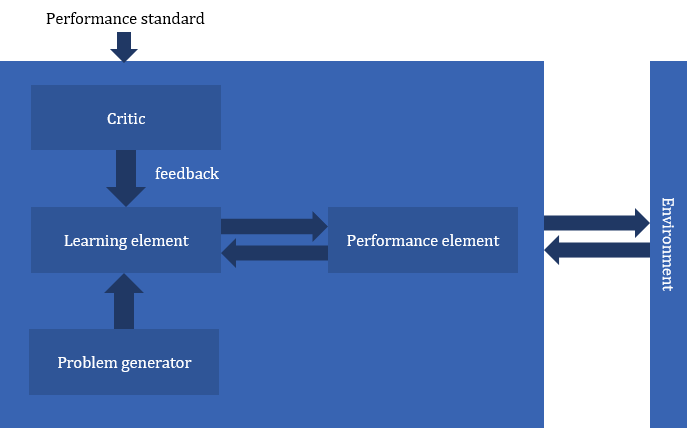
\includegraphics{aima_learning_agent}
    \centering
    \caption{An overview schematic of the learning agent system.}
    \label{fig:aima-learning-agent}
\end{figure}

\subsection{Learning and Performance}
The performance elements provides the basic function of the agent: it perceives, decides and acts.
The learning element's job is to improve this performance based on feedback, coming from an outside observer (the critic).
The learning element's design varies depending on the problem and how the agent is meant to interact with it.
One common example of implementation is a \emph{neural network}.
We will see how deep learning comes into play in Chapter \ref{deep-q-learning}.

\subsection{The Critic}
An agent cannot tell whether its behaviour is effective just by observing changes in the environment.
It needs a \textbf{critic} that provides feedback to the learning element about its performance in the world.
The critic can esentially be viewed as a stand-alone, external entity.
It is based on a fixed performance standard which does not depend on the agent's internal state.
In fact, it is imperative for the critic to be kept separate of agent state.
This prevents the agent of ``deluding'' itself that it is doing a good job.

\subsection{The Problem Generator}
Agents can get stuck making decisions that yield good but suboptimal results (local optima, a well-known problem in AI).
This happens because the agent bases its calculations on limited knowledge.
It needs a component to take care of adding new information into its system.
The problem generator solves this problem of \textbf{exploration}:
choosing options that yield suboptimal results in the short term, in order to discover better strategies on the long term.

\chapter{Elements of Reinforcement Learning} \label{reinforcement-learning}
\textbf{Reinforcement learning (RL)} is an area of machine learning that epitomizes the agent-based approach.
RL is unique within this field as it is directly focused on goal-directed learning from agent-environment interaction \cite{rlai}.
At the core of RL is the \emph{reward function}, which perfectly describes goals established by the problem.

RL is a class of problems as well as a class of solutions to those problems \cite{rlai}.
Despite the apparent \emph{supervised-unsupervised} split in machine learning, RL is cannot entirely fit in neither subset \cite{rlai}.

In the following chapter, we present the main concepts forming the framework of reinforcement learning.

\section{Feedback Loop}
First of all, we present the feedback loop, central to understanding the RL dynamic.
This is just a reiteration of the contents in our previous chapter:
an agent acts upon the environment, which reacts according to its set of governing rules.
The novel concept here is the \emph{reward signal}.
\begin{enumerate}
    \item The agent is in state \(s\) and picks action \(a\).
    \item It receives a reward \(r\) for its action. This (immediate) reward signal is problem-defined and quantifies the agent’s goal.
    \item The environment reacts, sending the agent into the next state \(s'\).
    \item The agent perceives \(s'\) and needs to decide on its next action.
\end{enumerate}

\begin{figure}[ht]
    \caption{The feedback loop in reinforcement learning. (Partial reproduction from \cite{rlai}, 3.2)}
    \centering
    \vspace*{0.5cm}
    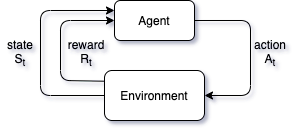
\includegraphics[width=0.5\textwidth]{agent-env-fig}
\end{figure}

Besides agent, reward and environment, we need to introduce several new concepts. A RL agent can be decomposed into state, policy, value function and (optionally) model \cite{rlai}.

\section{State and Policy}

The \textbf{state} most often refers to the internal state of the agent.
Although, in some contexts, we can use it to mean the environment state.
A state contains relevant information from the environment at a given time-step.
A key point in RL is that a well-engineered (agent) state captures all the relevant information and removes the need of explicitly memorizing state history.
This is mathematically by described the \textbf{Markov property} \cite{silver-lectures}, a fundamental property of the mathematical framework underpinning RL -- Markov decision processes (MDPs).

A \textbf{policy} completely characterizes the agent’s behaviour.
``It is a mapping from perceived states of the environment to actions to be taken in those states'' \cite{rlai}.
Policies can be deterministic (i.e. ``if this then that'' rules) or stochastic.
A \textbf{stochastic policy}\cite{silver-lectures} is a probability distribution over actions, given a state.

\section{Reward}
``The reward signal is the primary basis of altering the policy.'' \cite{rlai}.
The \textbf{reward} models the problem-defined goals as a scalar that can be associated with each state transition.
The assertion that we can completely and correctly model all goals using reward functions is central to the field of RL.
This is called the \textbf{Reward Hypothesis} and is formulated below:
\begin{quotation}
    That all of what we mean by goals and purposes can be well thought of as maximization of the expected value of the cumulative sum of a received scalar signal (called reward). \textit{(from \cite{rlai}, Chapter 3.2)}
\end{quotation}

The \textbf{return} denotes the cumulative reward obtained by the agent over time.
This is what a RL system is supposed to maximize.
There are multiple mathematical models used to represent the return.
The simplest example is to simply sum the reward over a finite number of steps.
However, in practice we often use \textbf{discounting}.
Discounting is, simply, a way to control how much the agent cares about future rewards.
More on this topic can be found in either theorethical reference \cite{rlai,silver-lectures}.
% In the actual paper, elaborate here.

\section{Value Function}\label{rl:value-func}

A \textbf{value function} measures how good each state is, with regard to the long-term potential of that state.
``Whereas rewards define the immediate desirability of an environmental state'', a value function ``indicates the long-term desirability of a state'' \cite{rlai}.
The value of a state is given by two things:
\begin{enumerate}
    \item the immediate value of being in that state (that state’s immediate reward)
    \item the potential return going forward in time from that state.
\end{enumerate}

This models a \textbf{long-term thinking aspect} into learning, as choosing one state over another often excludes future paths of action.
Let us take a game of chess as example.
If one move leads to the opponent capturing one of the agent's pieces, no future actions can be executed with that piece.
Thus, making a move with a high initial reward (for example, the agent trades a pawn for a knight), excludes -- for example -- the option of \textbf{promoting} that particular pawn (a later, higher reward).

\section{Model}
A RL system may or may not have a \textbf{model}.
A \textbf{model} (of the environment) allows the agent to plan and make predictions of its environment.

Some algorithms focus explicitly on learning a model and use it for \emph{planning}.
This approach is called \textbf{model-based}.
In this case, an agent can query the model to simulate what would happen with the environment, before actually choosing an action (hence the planning aspect).

Approaches without a model are called \textbf{model-free}.
Model-free agents are ``explicitly trial-and-error learners'' \cite{rlai}.

\begin{figure}[ht]
    \caption{A way of classifying RL methods based on whether they have a value function, policy or model. (Reproduced from David Silver's lectures. \cite{silver-lectures})}
    \vspace*{0.2cm}
    \centering
    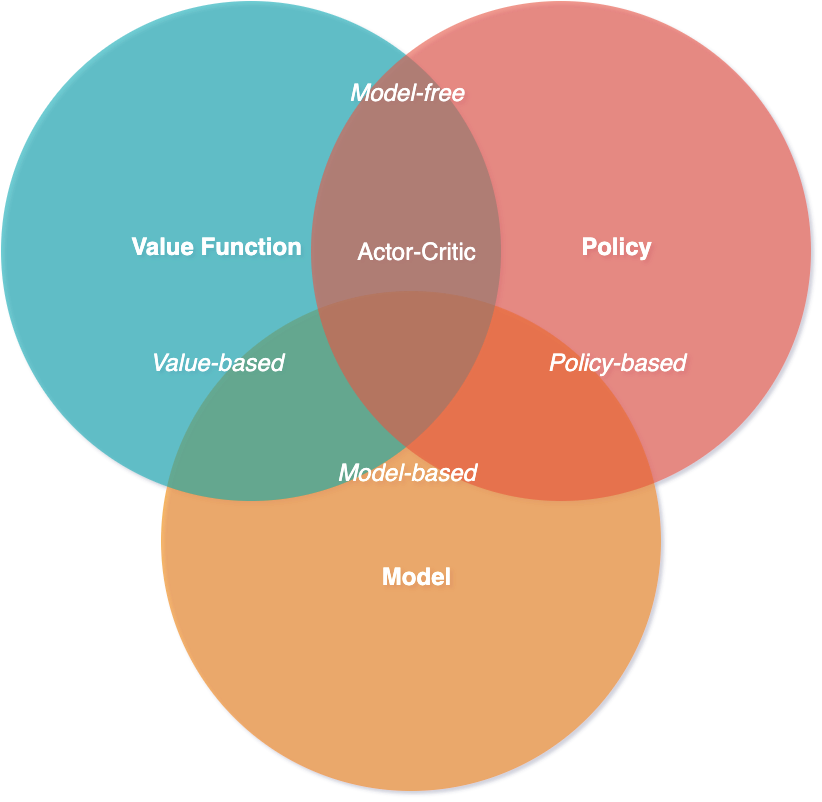
\includegraphics[width=0.5\textwidth]{silver-venn}
\end{figure}


\chapter{Deep Reinforcement Learning} \label{deep-reinforcement-learning}
Advances in the field of deep learning (a broad family of methods based on artificial neural networks \cite{wiki:Deep_learning}) were used to enhance the classical RL algorithms and led to the expansion of the field, marking the birth of \textbf{deep reinforcement learning (deep RL)}.
Deep RL has surged recently after a series of new algorithms and succesful applications were released.

In the following paragraphs, we will summarize some of the most significant results.

\textbf{AlphaGo} (2015) \cite{ago} managed superhuman performance in the game of Go, beating 18-time world champion Lee Sedol.
In late 2017, the AlphaGo family was expanded to contain AlphaGo Zero and AlphaZero\cite{alpha-zero}.
Both systems have managed to surpass all their predecessors in game performance, as well as training efficiency \cite{wiki:AlphaGo} (a lot less training time was required to beat the record).
The key difference was that their training was done with absolutely no expert knowledge for either system (hence the ``zero'').
Instead, everything was learned by self-play \cite{alpha-zero}.

\textit{Mnih et al.}'s \textbf{DQN} \cite{atari-dqn} (2013) managed impressive performance at seven classic Atari games.
The agents learn solely by observing the screen, without being given game-specific information.
This study produced agents able to surpass human-level performance in \emph{Breakout}, \emph{Enduro} and \emph{Pong}.
Following the success of DQN, the community worked to improve the standard algorithms, such as DDQN \cite{ddqn-paper} and PER \cite{per-paper}.
In Rainbow DQN (2017) \cite{rainbow-dqn}, the authors succesfully combined multiple high-quality improvement methods over the original DQN.
The resulting algorithm set a new record on the Atari benchmark.

\textbf{OpenAI Five} \cite{openai-dota} (2018) produced a bot that managed to beat top professional Dota 2 players in international championships.

In the following chapter, we will present an overview of the DQN method, as well as various improvements that enhance its performance.

\section{Q-learning and Q-networks}

Q-learning \cite{Watkins1992} appeared in 1992 and is considered one of the early breakthroughs of RL \cite{rlai}.
It is a simple algorithm allowing an agent to learn an optimal policy in an unknown environment.

Q-learning is part of \textbf{temporal difference (TD)} learning.
TD is a class of solution methods in RL that is part of the model-free subset \cite{rlai}.
An advantage of TD learning can learn from incomplete episodes \cite{long-peak-rl}.

\subsection{The Q-function}
In a Q-learning problem, the focus of our optimization is explicitly on actions, depending on the state they are taken in.
What we defined in \ref{rl:value-func} is a state-value function, as it maps each state to a value representing its desirability.
The Q function in Q-learning, in contrast, is an \emph{action-value function}.

An action-value function \(Q(s, a)\) (for ``quality'') takes a \emph{state-action pair} as input (not just a state).
Its value is the expected return of taking action \(a\) in state \(s\), then continuing to act based on the current policy.
This value can actually be decomposed into two parts: immediate reward \(r\) given by state \(s\), and the value of the successor state \({s}'\) \cite{silver-lectures}.
This idea is captured in the Bellman Equations, which we will omit here for brevity, but can be found in \cite{rlai, silver-lectures}.

A Q-learning agent chooses actions greedily based on their Q-values.
An optimal Q-function, denoted by  \(Q^{\star}(s, a)\), corresponds to an optimal policy (optimal behaviour for the agent).
Through the iterative process of Q-learning, our \(Q\) eventually converges to \(Q^{\star}\).

Q-learning is useful in problems with a finite number of states and a finite set of possible actions.
In the most trivial examples, the Q function can be represented as a table, memorizing state and action.

\subsection{(Deep) Q-networks}

Using a dictionary (data structure) to map state-action pairs to their values breaks down quickly in practice.
Instead, we need a more powerful model to store and update our Q-function.
A \textbf{neural network} can fill in the role of the function approximator.
This solves the data efficiency problem of Q-learning \cite{long-peak-rl}.
We call this a \textbf{Q-network}.
A \textbf{deep Q-network} has a multi-layered aspect.
``The Q-network can be a multi-layer dense neural network, a convolutional network, or a recurrent network, depending on the problem'' \cite{long-peak-rl}.

\section{Atari DQN}

Unfortunately, using a neural network to approximate the Q-function introduces additional complexity to the problem.
Whereas classical Q-learning is shown to be stable and manages to converge to the optimal values under easily-met conditions \cite{atari-dqn},
taking the Q-network approach may introduce \textbf{instability} and \textbf{divergence} \cite{long-peak-rl}.

\textbf{Atari DQN} \cite{atari-dqn} was used sucesfully to train RL agents on a set of seven classic Atari games, obtaining varying degrees of human performance on each.
The paper is considered a staple in the field of RL and Q-learning, and solved important problems with the original algorithm.

Atari DQN tackles the issues of Q-networks by introducing 
\textbf{experience replay}.

\subsection{Transition}

The papers discussed below define a \emph{transition} as the basic unit of agent-environment exchange.
A transition contains the observed initial state \(s\), the action \(a\) chosen by the agent and the reward \(r\), as well as the next state \(s'\). The definition of the state depends on the paper in question.
Usually, for the original DQN paper and its derivatives, a state consists of a short sequence of screenshots from the Atari emulator. The sequence length is four for the original DQN \cite{atari-dqn}.

\subsection{Experience Replay}

Experience replay refers to keeping a replay memory.
The replay memory stores all transitions observed during training.
In the approach described in \cite{atari-dqn}, the replay memory is used for sampling episodes at random.

The replay memory increments the sample efficiency of Q-learning.
Q-learning is an \emph{online} learning algorithm: given a sample, it will consume it immediately to adjust its values.
This process of instantly discarding samples can lead to ``forgetting''.
Storing every sample overcomes this problem.

Random sampling is important due to the nature of the data.
To explain why replay grants a significant advantage, let us consider a more popular use-case for neural networks: classification problems.
In supervised learning, a correct training set contains samples that are \emph{uniformly distribuited}.
Our problem differs significanlty in definition: our input data is sequential.
Game states obtained from the Atari emulator are highly correlated.
Using highly correlated data to train our Q-network can easily lead to overfitting \cite{jaromiru-dqn}.
Thus, it is better to sample episodes at random instead of training in an ordered sequence.

In DQN, the capacity of the replay memory is limited, as specified by a hyperparameter \(N\). When the memory is full, it discards the oldest sample.

\section{DDQN: Double Deep Q-networks}
The DQN approach is prone to be overly optimistic when it comes to the estimated Q-values.
A DQN agent eventually reaches a peak in performance.
The experience memory becomes polluted with overwhelmingly positive experiences, which in turn, destroy the quality of the Q-newtork.

The \textbf{Double DQN} \cite{ddqn-paper} approach attempts to correct the overestimation problem.
It proposes using two neural networks to predict the action at every time-step.

\subsection{Target Network}

In Q-learning, the \(Q\) function is updated based on its own values.
In a Q-network, this would translate to updating the network based on its own parameters. This can introduce instability and divergence \cite{jaromiru-dqn}.

The idea of a target network is simple in principle:
every \(t\) time-steps, we take a snapshot of the main network's parameters and use them to create a \textbf{target network}.
The target network is \emph{frozen} \cite{long-peak-rl} until the next snapshot.
Between snapshots, \(Q\) is optimized based on values of the target.
This significanlty reduces oscillations, increasing stability of learning \cite{atari-dqn}.

\section{PER: Prioritized Experience Replay}

Another improvement is given by \emph{Schaul et al.} in the \emph{Prioritized Experience Replay} paper \cite{per-paper}.

Recall that in the original DQN, episodes are uniformly sampled from the experience memory.
This causes a problem when our agent is doing well.
Our memory quickly fills up exclusively with successful states.
The replay memory automatically discards the older samples as the new ones pile up and the DQN system stops learning.

In this paper, researchers acknowledge that not all samples have equal learning value for the system.
Thus, ranking samples according to their significance should improve the efficiency of learning.

Several approaches to prioritizing replay samples are presented in \cite{per-paper}. In the section below we attempt to shortly summarize \textbf{proportional prioritization}.

\subsection{Proportional Prioritization}

This strategy proposes ranking each transition proportional to its error.

The \emph{error} is the difference between the \(Q_{\star}(s, a)\)  value (predicted by the online Q-network) and the target estimate (predicted of the target network).

The main idea of this approach is that we assume that our system can learn more efficiently from those divergent states.
The higher the error of a transition, the more it diverges from the Q-network's predictions.
We know, intuitively, that humans (and animals) also learn efficiently from experiences which contradict our expectations.

\chapter{Our Approach}
In this chapter, we focus on \emph{Pac-Man} as learning environment and on our collection of agent programs based on deep Q-learning.

The project itself consists of a light framework for training, running and evaluating RL agents.
Our framework is compatible with various other environments, as long as they respect the interface provided by OpenAI Gym.
The feature set includes automatic checkpoints, cloud-friendly deployment and a performance analysis toolkit.

In Section \ref{section:modelling-the-problem}, we justify why we choose to study the game of \emph{Pac-Man} and formalize the specifications of it as a learning environment.

In Section \ref{section:approach-algorithms}, we introduce some of the algorithms built into our collection of autonomous agents.
The main method is vanilla DQN, which was covered previously in Section \ref{section:dqn}.
However, in this section, we present two important improvements over it -- double DQN and Prioritized Experience Replay.

In Section \ref{section:implementation}, we take a look at each subcomponent of an individual agent program and map each one to notions from our previous chapter.
Each agent has its own module and inherits a specific structure from a prototype.

In Section \ref{section:technologies}, we present a rundown of our technology stack, whose core is the Python programming language. The framework is built on the PyTorch machine learning library but makes use of many other ML and data science libraries.

We wrap up this chapter with Section \ref{section:user-manual} which consists of a short instruction manual for users to start local or remote training sessions, use the provided performance measurement tools and extend the existing collection of agents.

\clearpage

\section{Modelling the Problem} \label{section:modelling-the-problem}
The problem we solve in this thesis is three-fold.
Firstly, we specify a variant of a task environment for \emph{Pac-Man}, defining goals and rewards to view it through the lens of reinforcement learning.
Secondly, we train agents to ``solve’’ that environment, i.e. explore and learn to take optimal decisions to achieve the established goals.
And lastly, we compare agents based on proximity to their goals, mean reward and learning stability.

\textbf{\textit{Pac-Man}} is a classic video game developed by Toru Iwatani and published by Namco Ltd. in 1980 \cite{pacman-in-academia}.
The game was originally released as an arcade game and it quickly became the most commercially sucessful arcade game ever created.
The original hit gave rise to a series of ``licensed clones'', which targeted a number of popular platforms, such as the Atari 2600, the Nintendo Entertainment System (NES), the Nintendo GameBoy, etc.
Besides its commercial success, \emph{Pac-Man} has been an appealing object of study for academia, across a number of fields, ranging from psychology to mathematics and computational intelligence \cite{pacman-in-academia}.

\begin{figure}[h]
    \centering
    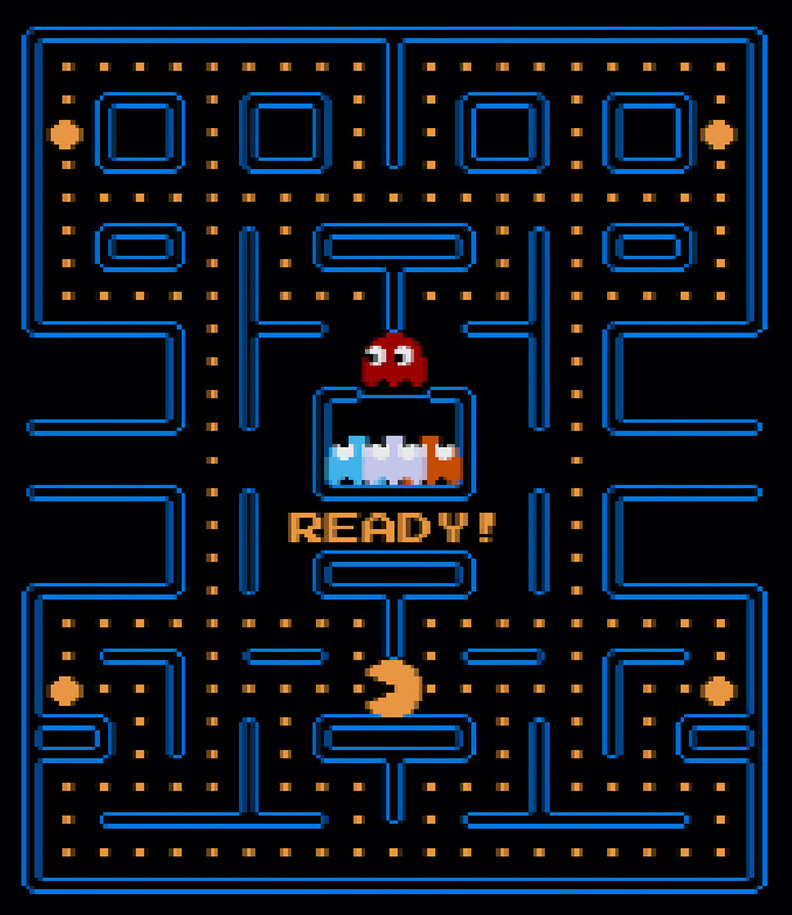
\includegraphics[width=0.4\textwidth]{nes-pac-man.jpg}
    \caption{Screen capture of the starting configuration from Nintendo's NES variant of the game.}
    \label{fig:pac-man-screen}
\end{figure}

The game's mechanics are intuitive but engaging enough to be fun.
It allows simple four-directional movement.
The player is represented as a yellow character with a distinctive circular shape (with a ``missing slice''\footnotemark{} representing its mouth).
\footnotetext{Iwatani's stated inspiration for Pac-Man's design was a pizza with a missing slice. \cite{pacman-gameinformer}}
The board is a bidimensional maze, featuring tunnels which loop around each other, i.e. entering a tunnel on one side will transport the player out through the opposite side of the board.
\textbf{Pellets} (or \emph{dots}) are placed at almost every position, and the goal of every level is to collect all pellets.
Most renditions of the game feature four \textbf{ghosts} which will chase the player around the board.
Collisioning with any of the ghosts results in losing a life and being repositioned to the start (without losing progress on dots).
The ghosts have different ``personalities'' -- each of them has a different approach for chasing Pac-Man.
There are special power pellets in each of the four corners (seen in Figure \ref{fig:pac-man-screen}).
\textbf{Power pellets} grant Pac-Man temporary immunity from ghosts and changes the power dynamic in the game for a short time: the ghosts enter \textbf{``scared'' mode} and reverse their direction to run away.
In this mode, the player gets an increasing score for every ghost it eats.

\emph{Pac-Man} can be defined as a 2D gridworld environment, where exploration is necessary to reach the goal.
This class of task environments is common throughout RL literature and has some common properties:
\begin{itemize}
    \item they have discrete bidimensional representation;
    \item an agent has a finite set of options at every time step.
\end{itemize}

\textbf{Gridwords} are used in literature to clearly define and \textbf{isolate} agent goals.
A simplistic environment with a clear task is also beneficial for agent learning due to its low degree of environmental noise -- the agent can ``focus'' on the task.
The ease of customizability of the rules inside a gridworld allows creating interesting strategy games to test agents’ decision-making capabilities.
New non-trivial grid-based environments are an area of open research -- for example, the \emph{Pommerman} benchmark \cite{pommerman-paper} has been formulated as a novel interesting multi-agent problem which does not yet have an optimal solution.

\emph{Pac-Man} has a few advantages which make it interesting to study from a RL perspective.

First of all, it provides a \textbf{shaped reward} built-into the game mechanics.
In reinforcement learning, a \textbf{sparse reward} is a large reward which is delayed for a relatively large number of steps.
A sparse reward would be, for example, if we would only reward the agent at the end of the game.
Shaped rewards, in contrast, equate with providing gradual feedback to the agent.
This can improve learning and lead to better outcomes earlier in training, as good behaviours become immediately obvious to the agent.

In \emph{Pac-Man}, the pellets, placed uniformly over the board, provide a shaped reward which directly reflects the goal of the game, i.e. to eat all pellets on a board without getting caught.
Moreover, they \textbf{incentivize exploration} as the reward is higher in places the agent has not visited before.

Second of all, \emph{Pac-Man} requires the agent to develop non-trivial strategies.
The game requires balancing two equally important subgoals: fully covering the game board to consume every available pellet, and running away from the chasing ghosts.
This gives rise to complex and potentially problematic situations for the player, which require \textbf{planning}.
This raises an interesting question regarding the potential of existing algorithms to learn \textbf{long-term strategies} similar in performance to human players.

The \textbf{reward function} we use in this thesis for our \emph{Pac-Man} environment is a combination of a few properties of the environment state.
The most important component is the \textbf{score}.
Score changes will determine a proportional reward for the agent.
Significant score increases are provided by eating pellets but a more interesting mechanic is eating ghosts when the player is invincible.
Each ghost eaten will provide a higher reward, thus conditioning the agent to chain as many ``kills'' as possible.
Typical of arcade games, the mechanics are built such that the score can \emph{only increase} over time.
This creates a necessity to \emph{counterbalance} by finding opportunities for \textbf{punishment}.
We choose to strongly penalize the agent for losing a life.
There are other possible candidates for ``punishment'' events, but we consider ``death on ghost contact'' to be the most important for capturing the goal of the game.

\section{Algorithms} \label{section:approach-algorithms}
In this section, we present the main algorithms powering the autonomous agents evaluated in this thesis. In our collection, \textbf{vanilla DQN} serves both as a stand-alone implementation, as well as a fundamental building block of more advanced algorithms.
The original DQN, however, is already covered by Section \ref{section:dqn} of our theory chapter and we will omit it here for conciseness.
Instead, this section deals with \textbf{double DQN} and \textbf{prioritized experience replay (PER)}, both of which address shortcomings of the original algorithm.

\subsection{Double Q-learning} \label{section:double-dqn}
Double DQN \cite{ddqn-paper} is an algorithm in the deep Q-learning family, discovered and published by DeepMind researcher Hado van Hasselt along with several other colleagues.
The study determines that general Q-learning (and, by extension, deep Q-learning) suffers from a problem known as a \textbf{maximization bias} and adapts the original algorithm to account for this and counteract the bias.

Stated simply, a \textbf{maximization bias} is an implicit preference of the algorithm to overestimate values, despite divergence from the true value.
Some control algorithms, such as Q-learning, fundamentally depend on using the maximum over estimated values as an estimate for the maximum value \cite{rlai}.
This leads to situations where noisy reward signals, prevalent in real-world environments, can significantly destabilize learning and slow down training progress.

Hasselt proposes \emph{double learning} to counteract this bias.
This requires two independent approximators of the action-value function -- we will denote them $Q_1$ and $Q_2$.
At every step, the approximators are \emph{intermittently} used either to pick an action or to estimate its value.
The paper proves that this decoupling is sufficient to accomplish an unbiased estimation.
Which function serves which role can be chosen uniformly at random at every learning step at practically no cost.
Equation \ref{eqn:double-learning-rule} states the double learning \textbf{update rule}, considering the situation in which $Q_1$ picks the action (and is updated) while $Q_2$ gives the estimate which we bootstrap from.

\begin{equation} \label{eqn:double-learning-rule}
\begin{aligned}
Q_1(S_t, A_t) & \leftarrow Q_1(S_t, A_t) \\
    & + \alpha [ R_{t+1} + \gamma Q_2(S_{t+1}, \argmax_{a \in A} Q_1(S_{t+1}, a)) - Q_1(S_t, A_t)]
\end{aligned}
\end{equation}

A drawback of the double learning algorithm is that it requires double the amount of memory of the original. 
Despite this, it still performs one update per step, so the running time is equivalent to that of its predecessor.
% to steal more content space, include and explain the example from RLAI

\subsection{Prioritized Experience Replay (PER)} \label{section:per}
\textbf{Prioritized experience replay} (often shortened as \emph{PER}) is an extension of deep Q-learning, also developed by a team at DeepMind, led by Tom Schaul \cite{per-paper}.
The paper focuses on improving experience replay from classic DQN.

Recall from Section \ref{section:dqn} the principle of \textbf{experience replay}, which consists of storing all transitions the agent experiences in order to revisit them later during training.
Reusing experiences over multiple update steps reduces the number of samples required for learning.
The original approach suggests that the experiences are revisited by sampling them uniformly at random from the replay memory.
This has the important role of \emph{decoupling} experiences -- which in the case of successive video game frames, are by nature highly correlated -- to avoid introducing \emph{high variance} into the system (which can cause overfitting).

The foundational hypothesis of the paper at \cite{per-paper} is that some transitions have higher ``teaching’’ potential than others.
The \emph{prioritization} mentioned in the title refers to finding an ordering over experiences which properly reflects this potential.
The authors chose \emph{absolute TD-error} as a good approximation for utility in learning -- for several reasons.
Firstly, since larger errors suggests that a prediction is further from the agent’s current expectations, minimizing larger errors would naturally improve performance the most.
This supposition has intuitive appeal because \textbf{humans} likewise learn proportionally more from experiences that contradict their existing beliefs the most.
Additionally, TD-error is already computed as part of the normal update cycle in DQN so extending the implementation to PER does not require significant overhaul of the algorithm.

The paper develops two separate models for prioritizing experience based on error.
Each model specifies how priorities are computed and stored.

\textbf{Rank-based prioritization} involves keeping track of the rank each transition occupies.
Each transition would thus have an assigned priority of $p = 1 / rank$.
This requires an additional data structure, capable of online sorting, such as a heap, as some ranks will change at every update step.

Since the replay memory can potentially store millions of transitions, \textbf{optimization} is necessary to prevent severely hindering performance.
Changing every rank at every update step is impractical and would outweigh the benefits of prioritization.
In order to mitigate this, the authors propose to only re-evaluate the ranks of transitions in the sampled mini-batch.
This \textbf{``lazy’’ approach} retains its desirable properties of learning more efficiently than DQN while not adding an insane amount of computation.

\textbf{Proportional prioritization} simply assigns a priority equal to the absolute TD-error plus an $\epsilon$: $p_{i} = |\delta_{i}| + \epsilon$.
The $\epsilon$ (which should not be confused with our exploration coefficient in $\epsilon$-greedy) is an offset keeping all priorities above $0$.

The second part of the algorithm is common to both models and consists of actually assigning probabilities based on priority and building the distribution over the transitions. The formula in (\ref{eqn:per-probability}) gives an outline of the method.

\begin{equation} \label{eqn:per-probability}
    P(i) =  \left( \frac{p_i}{\sum_{k}{p_{k}}} \right)^\alpha
\end{equation}

The $\alpha$ parameter in this equation represents the degree of prioritization, i.e. a higher $\alpha$ will determine a larger difference between the probabilities of any two consecutive transitions (when ordered by priority).

To sample according to the obtained distribuition, a sum tree is used.
A \textbf{sum tree} is a specialized type of segment tree -- a tree data structure which stores \emph{statistics} (e.g. minimum, maximum, sum etc.) of its leaf nodes.
The values of the leaf nodes are usually stored in an array.
The structure is designed to compute interval queries over that array, such as the sum of all values between indices $x$ an $y$, in $\mathcal{O}(\log{n})$, while also allowing fast updates to the underlying data.

\section{Implementation} \label{section:implementation}
The models and algorithms presented throughout our theory chapter and in the previous section are incorporated into our framework and implemented using Python and the PyTorch machine learning library.
The framework is divided into several modules which we detail below.

The \verb|common| package contains classes which are shared among all agent implementations, including those concerning training and evaluation, but also configuration, and a checkpoint manager.

Each agent implementation has its own package: \verb|deepq| is the vanilla DQN agent, \verb|per| implements prioritized experience replay on top of the default DQN, and \verb|doubledqn| and \verb|doubleper| are the double Q-learning versions of the former two.
We cover them in Section \ref{section:agent-modules}.

The \verb|replay_memory| package contains the logic used for memorizing transitions (units of agent experience).
This package is used by all agents to store, sample and replay transitions.
We are keeping it isolated because it is clearly logically separate and because it is complex on its own.

\verb|ds| is short for ``data structures'' and contains our implementation of the sum tree required by \verb|replay_memory.PrioritizedReplayMemory|.

The \verb|wrappers| package contains a helper class which works as a layer on top of OpenAI Gym to implement a few missing features required to properly run and test agents according to the original papers.

While not a package per se, but kept separately from our training logic, we have our Jupyter notebooks (in \verb|notebooks|).
We use those to analyze scores, to graph and benchmark agent performance.
Inside this directory is an isolated \verb|plot| package, custom-built to allow us to work with both data gathered from either a single run or from multiple runs of the same configuration -- this logic is encapsulated in the \verb|SingleRunData| and \verb|MultiRunData| classes.

\subsection{\texttt{Trainer} and \texttt{Evaluator}}

\begin{figure}[ht]
    \centering
    \begin{subfigure}[b]{0.5\textwidth}
        \centering
        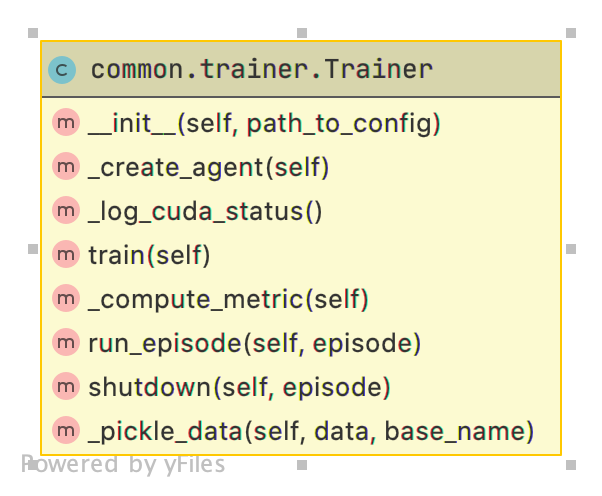
\includegraphics[width=0.5\textwidth]{app-trainer.png}
        \caption{Class diagram of \texttt{Trainer}.}
        \label{fig:trainer-diagram}
    \end{subfigure}%
    \hfill
    \begin{subfigure}[b]{0.5\textwidth}
        \centering
        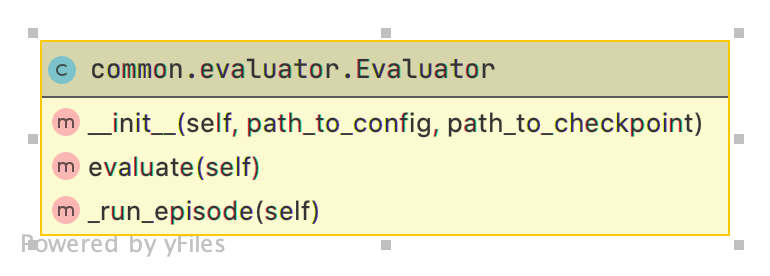
\includegraphics[width=0.5\textwidth]{app-evaluator.png}
        \caption{Class diagram of \texttt{Evaluator}.}
        \label{fig:evaluator-diagram}
    \end{subfigure}
\end{figure}

\texttt{Trainer} and \texttt{Evaluator} host the main loop and constitute (separate) entry points into the system.
The \textbf{trainer} can differ between algorithms and contains more complex procedures overall.
The \textbf{evaluator} is roughly doing the same thing, but is more universal as it does not need to encapsulate any algorithm-specific logic.

Both systems start by loading the configuration file using the \texttt{ConfigLoader}.
This is a simple utility class which loads a \texttt{YAML} file into memory.
After the data is loaded, each level has the responsibility to parse it according to its requirements.
For example, we generally group hyperparameter data under the \texttt{model} category of a configuration file, representing parameters required to calibrate the algorithm.
The trainer's job is \textbf{general} -- to redirect the model parameters to the agent -- and thus does not do any parsing by itself.
It is the agent’s job to parse and validate the data.

For training, we initialize every needed component: agent, environment, checkpoint manager, etc.
The main loop consists of fetching the current state from the emulator, feeding it to the agent for learning and processing, then playing the agent’s chosen action into the emulator.
At every iteration, we log scores, compute statistics for plotting and call the checkpoint manager to check if the current state needs to be saved.
An activity diagram of the training process is provided in Figure \ref{fig:training-loop-activity-diagram}.

\begin{figure}[h]
    \centering
    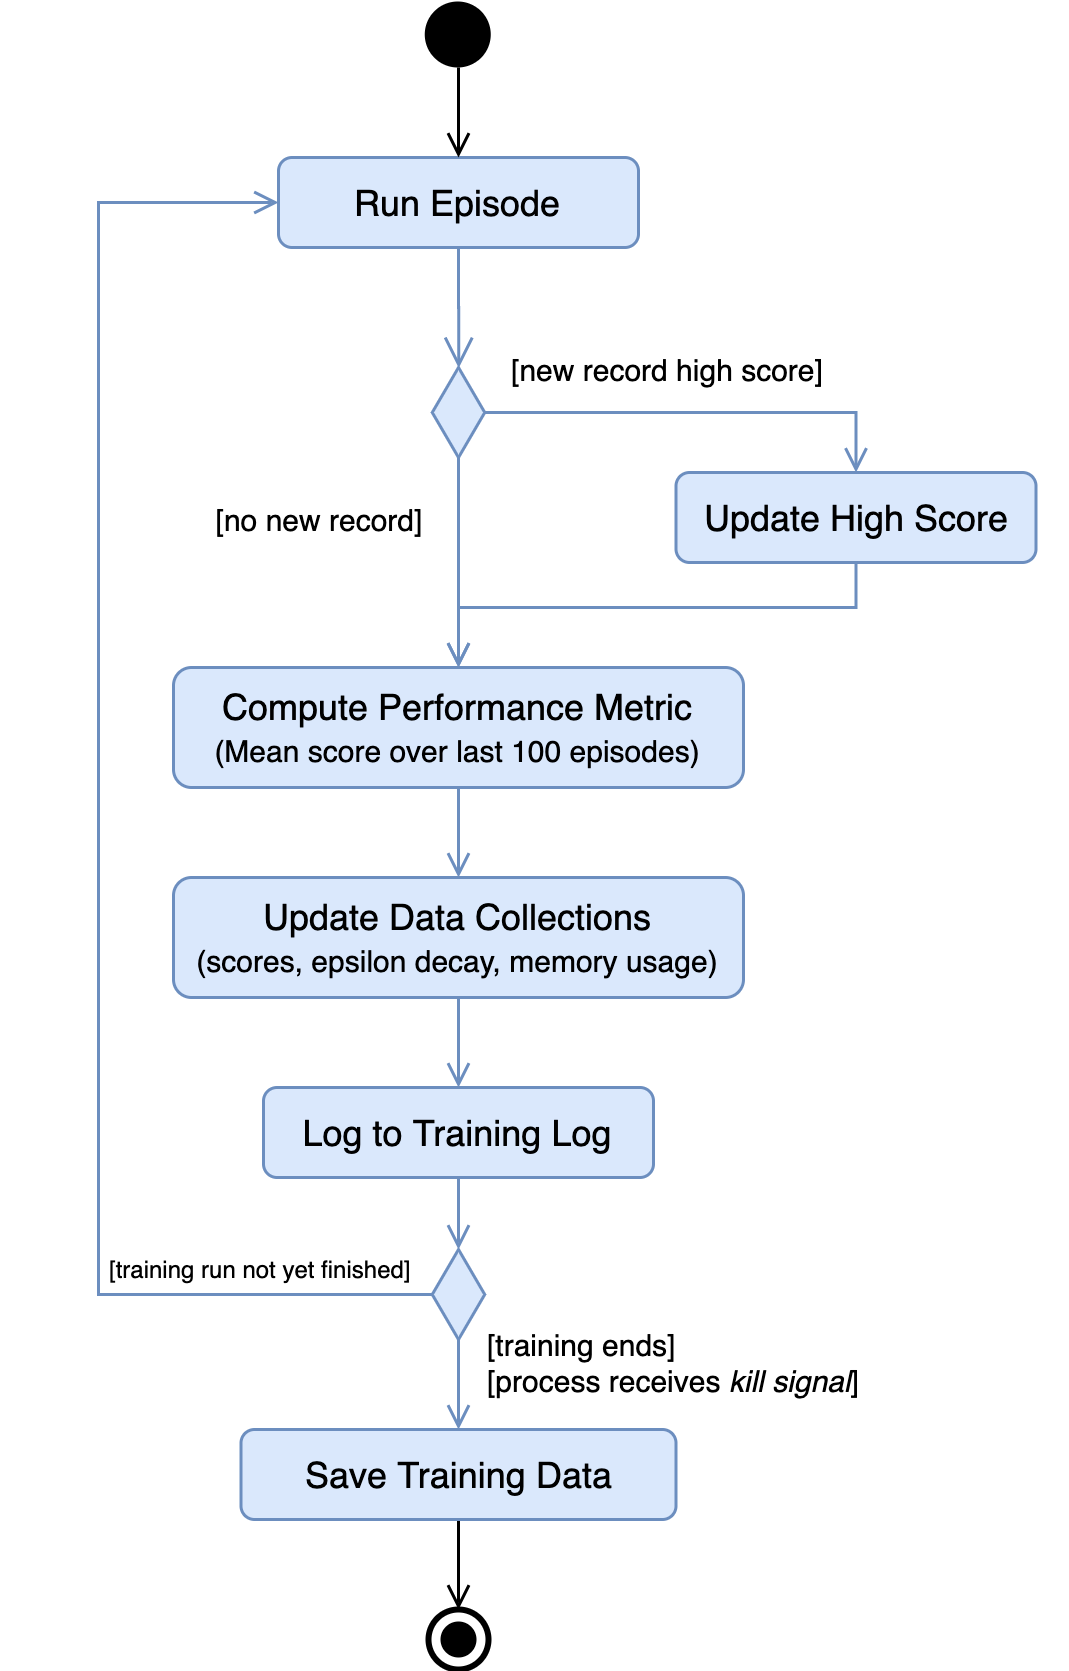
\includegraphics[width=0.6\textwidth]{training_activity_diagram.png}
    \caption{Activity diagram of the main training loop in our \texttt{train()} function.}
    \label{fig:training-loop-activity-diagram}
\end{figure}

\begin{figure}
    \centering
    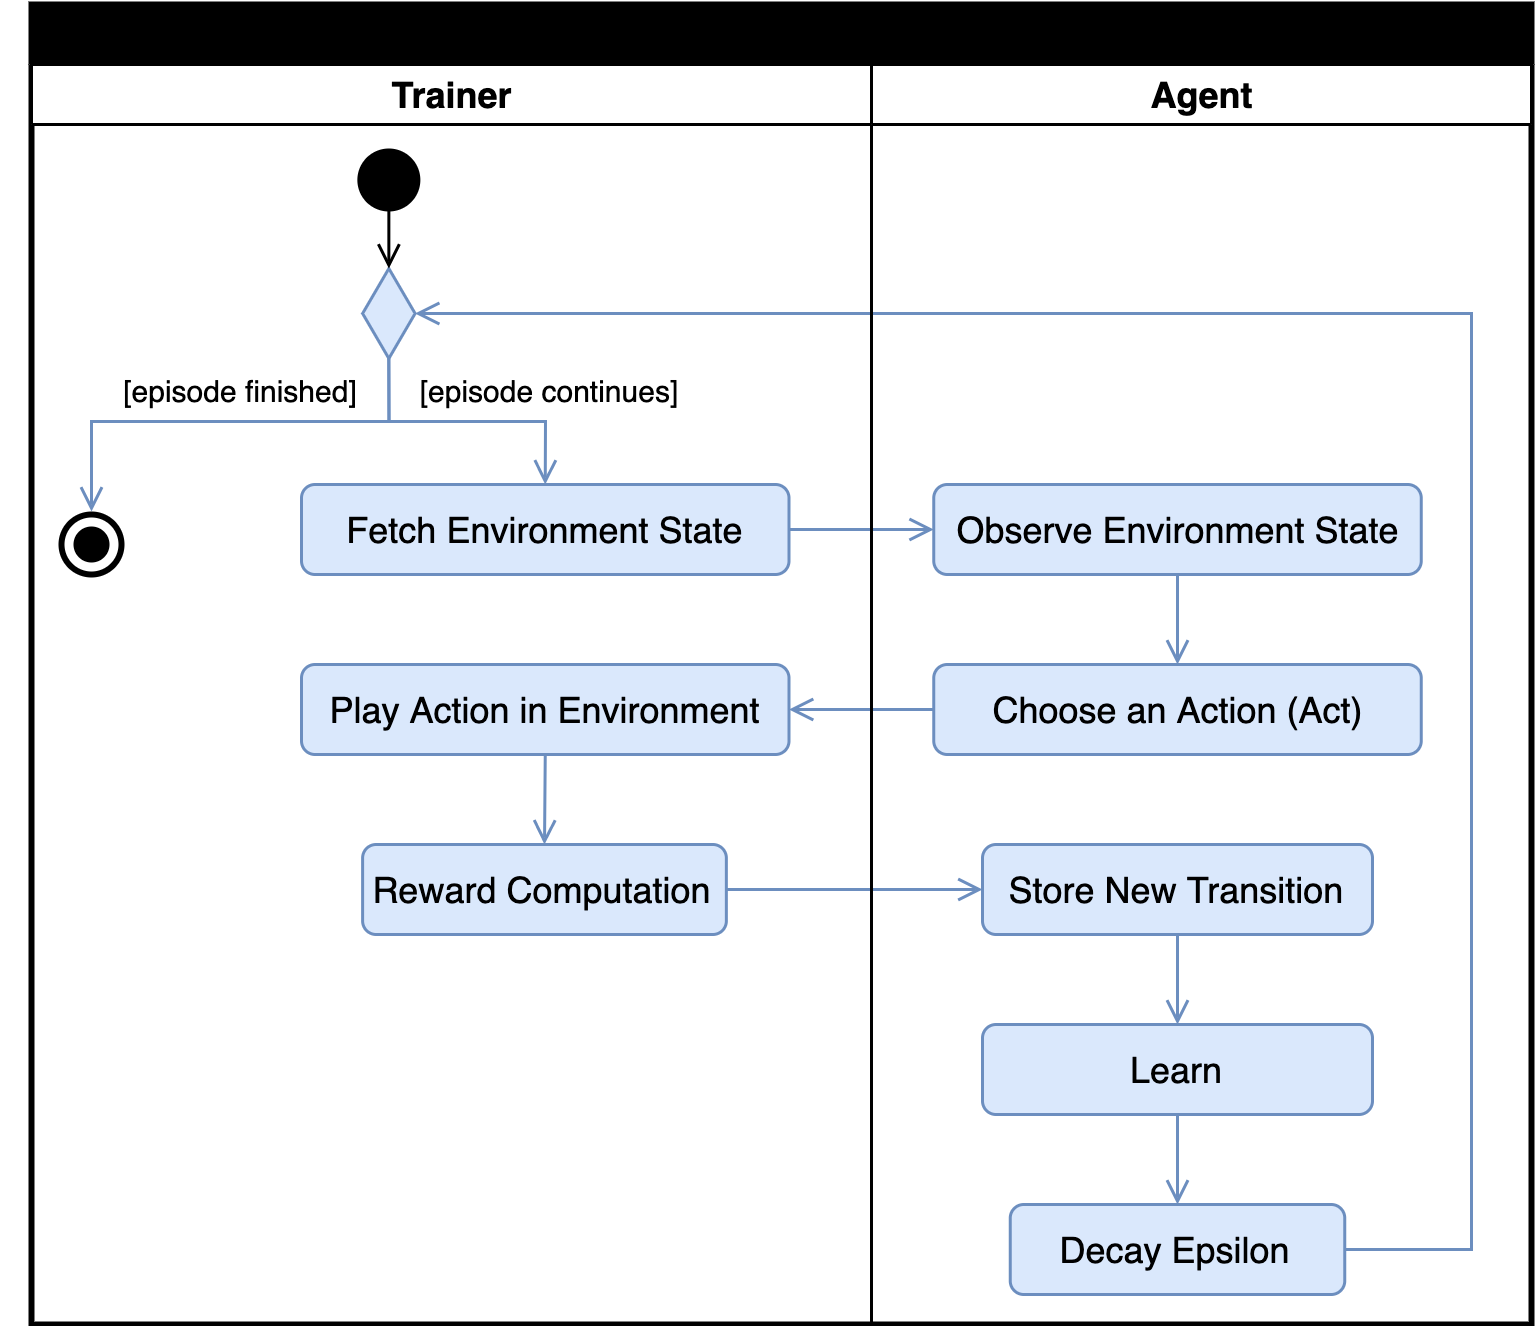
\includegraphics[width=\textwidth]{run_episode_activity_diagram.png}
    \caption{An activity diagram corresponding to the ``Run Episode'' sub-task from Figure \ref{fig:training-loop-activity-diagram}. This diagram highlights the agent-environment loop.}
    \label{fig:run-episode-diagram}
\end{figure}

The \texttt{Trainer} class has a \emph{graceful exit} procedure, the \texttt{shutdown} method.
It is triggered automatically at the end of training and mapped to the \texttt{SIGKILL} signal.
Training jobs are designed to be able to run for a long time inside a cloud instance, including on preemptible instances\footnotemark{}.
\footnotetext{relatively low-cost instances which can be terminated at any time if required by the cloud provider.}
The procedure consists of checkpointing the model, saving statistics (scores, epsilon decay data and memory usage) and compresses everything into a file before terminating.

The \textbf{evaluator} essentially does the same thing as the trainer, without accounting for checkpointing or agent learning.
It simply executes as many evaluation runs as specified by the configuration file and saves the statistics.
An distinguishing feature of the evaluator is that it captures video from inside the emulator and saves it at the location specified in \texttt{monitor.path}.

\subsection{\texttt{CheckpointManager}}

\begin{figure}[ht]
    \centering
    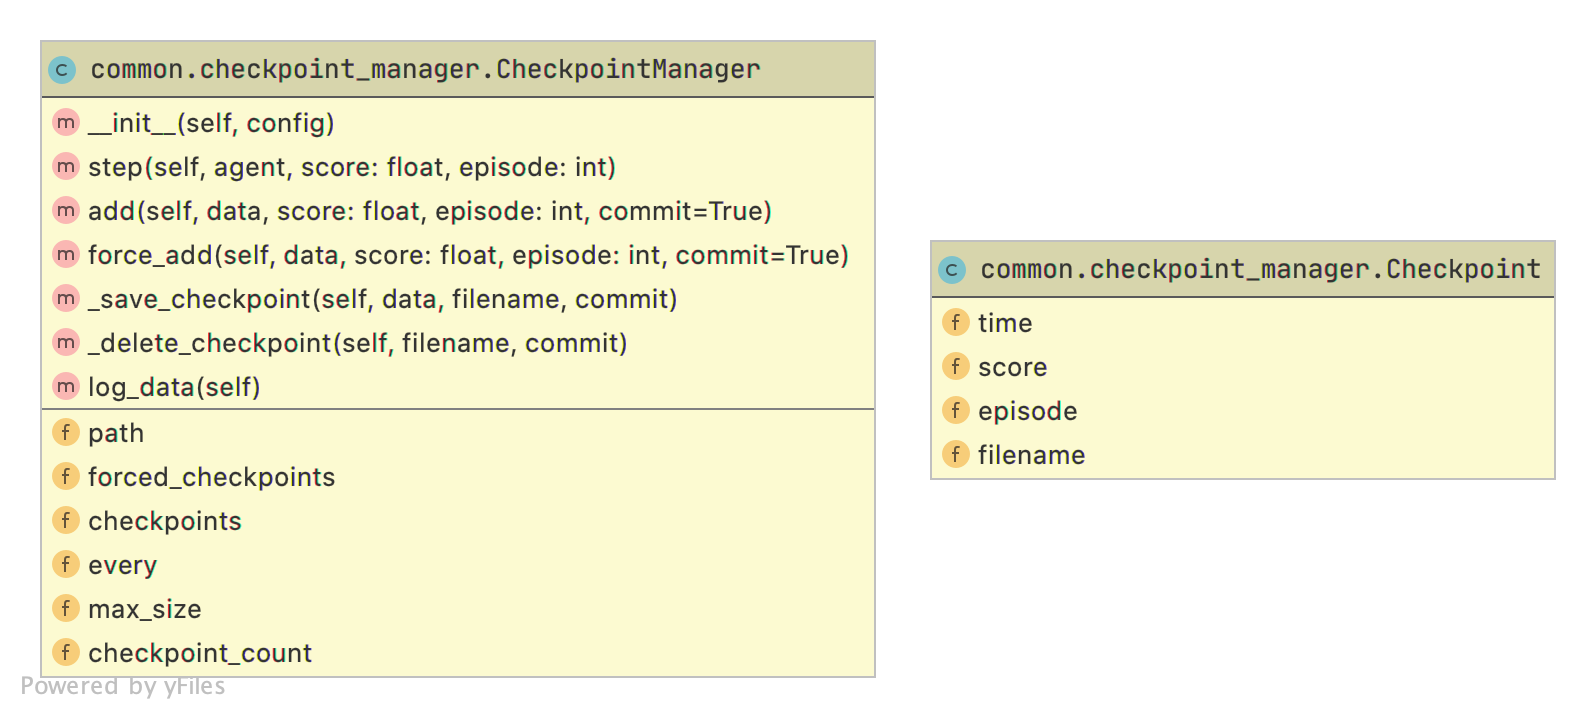
\includegraphics[width=0.7\textwidth]{app-checkpoint-manager.png}
    \caption{The class diagram of \texttt{CheckpointManager}, next to \texttt{Checkpoint}.}
    \label{fig:checkpoint-manager}
\end{figure}

\texttt{CheckpointManager} is a utility class whose purpose is to periodically capture snapshots of the agent model (the neural networks), along with other metadata (training epoch, hyperparameters, etc.) during training.
The best snapshots from training are used to reconstruct the agent and play the game in the evaluation environment.

Each snapshot file is several megabytes in size and a proper training session usually runs for hundreds of thousands (ideally, millions) of training steps.
In order to conserve disk space during training, the job of the checkpoint manager is to always compare the snapshots based on a predetermined metric in order to decide which ones to keep and which ones to remove.
The default metric used in this implementation is the average score over the last 100 episodes (an episode in the context of Pac-Man means a full level playthrough from board initialization until a terminal state is reached).

A separate \textbf{``forced'' checkpoint} is taken at the end of training, regardless of the score metric.
This is done because most algorithms don’t stabilize until the very end of training.
However, despite more reliably reaching good scores, well-performing agents do sometimes score lower than previous record high-scores induced by earlier local optima or by chance.

The manager is configurable -- its adjustable properties are the checkpoint frequency \texttt{every}, 
representing the number of steps between two consecutive snapshots, and the allowed capacity
\verb|max_size|, the maximum number of files it can store during a training run.

\subsection{Agent Modules} \label{section:agent-modules}

The framework contains a collection of agents, currently consisting of four different algorithms in the DQN family.
The relations among the agent classes is detailed in Figure \ref{fig:agent-class-diagram}.

\begin{figure}[h]
    \centering
    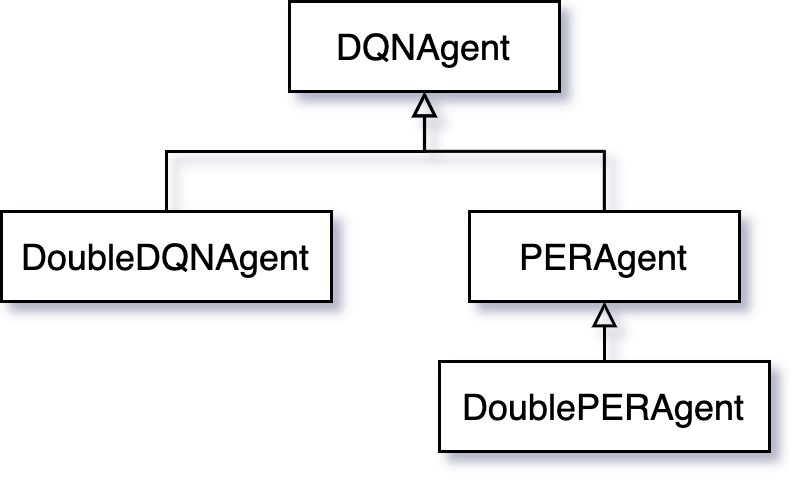
\includegraphics[width=0.5\textwidth]{app-agent-inheritance-diagram.png}
    \caption{A diagram representing the agent classes and their inheritance relations.}
    \label{fig:agent-class-diagram}
\end{figure}

\begin{figure}[h]
    \centering
    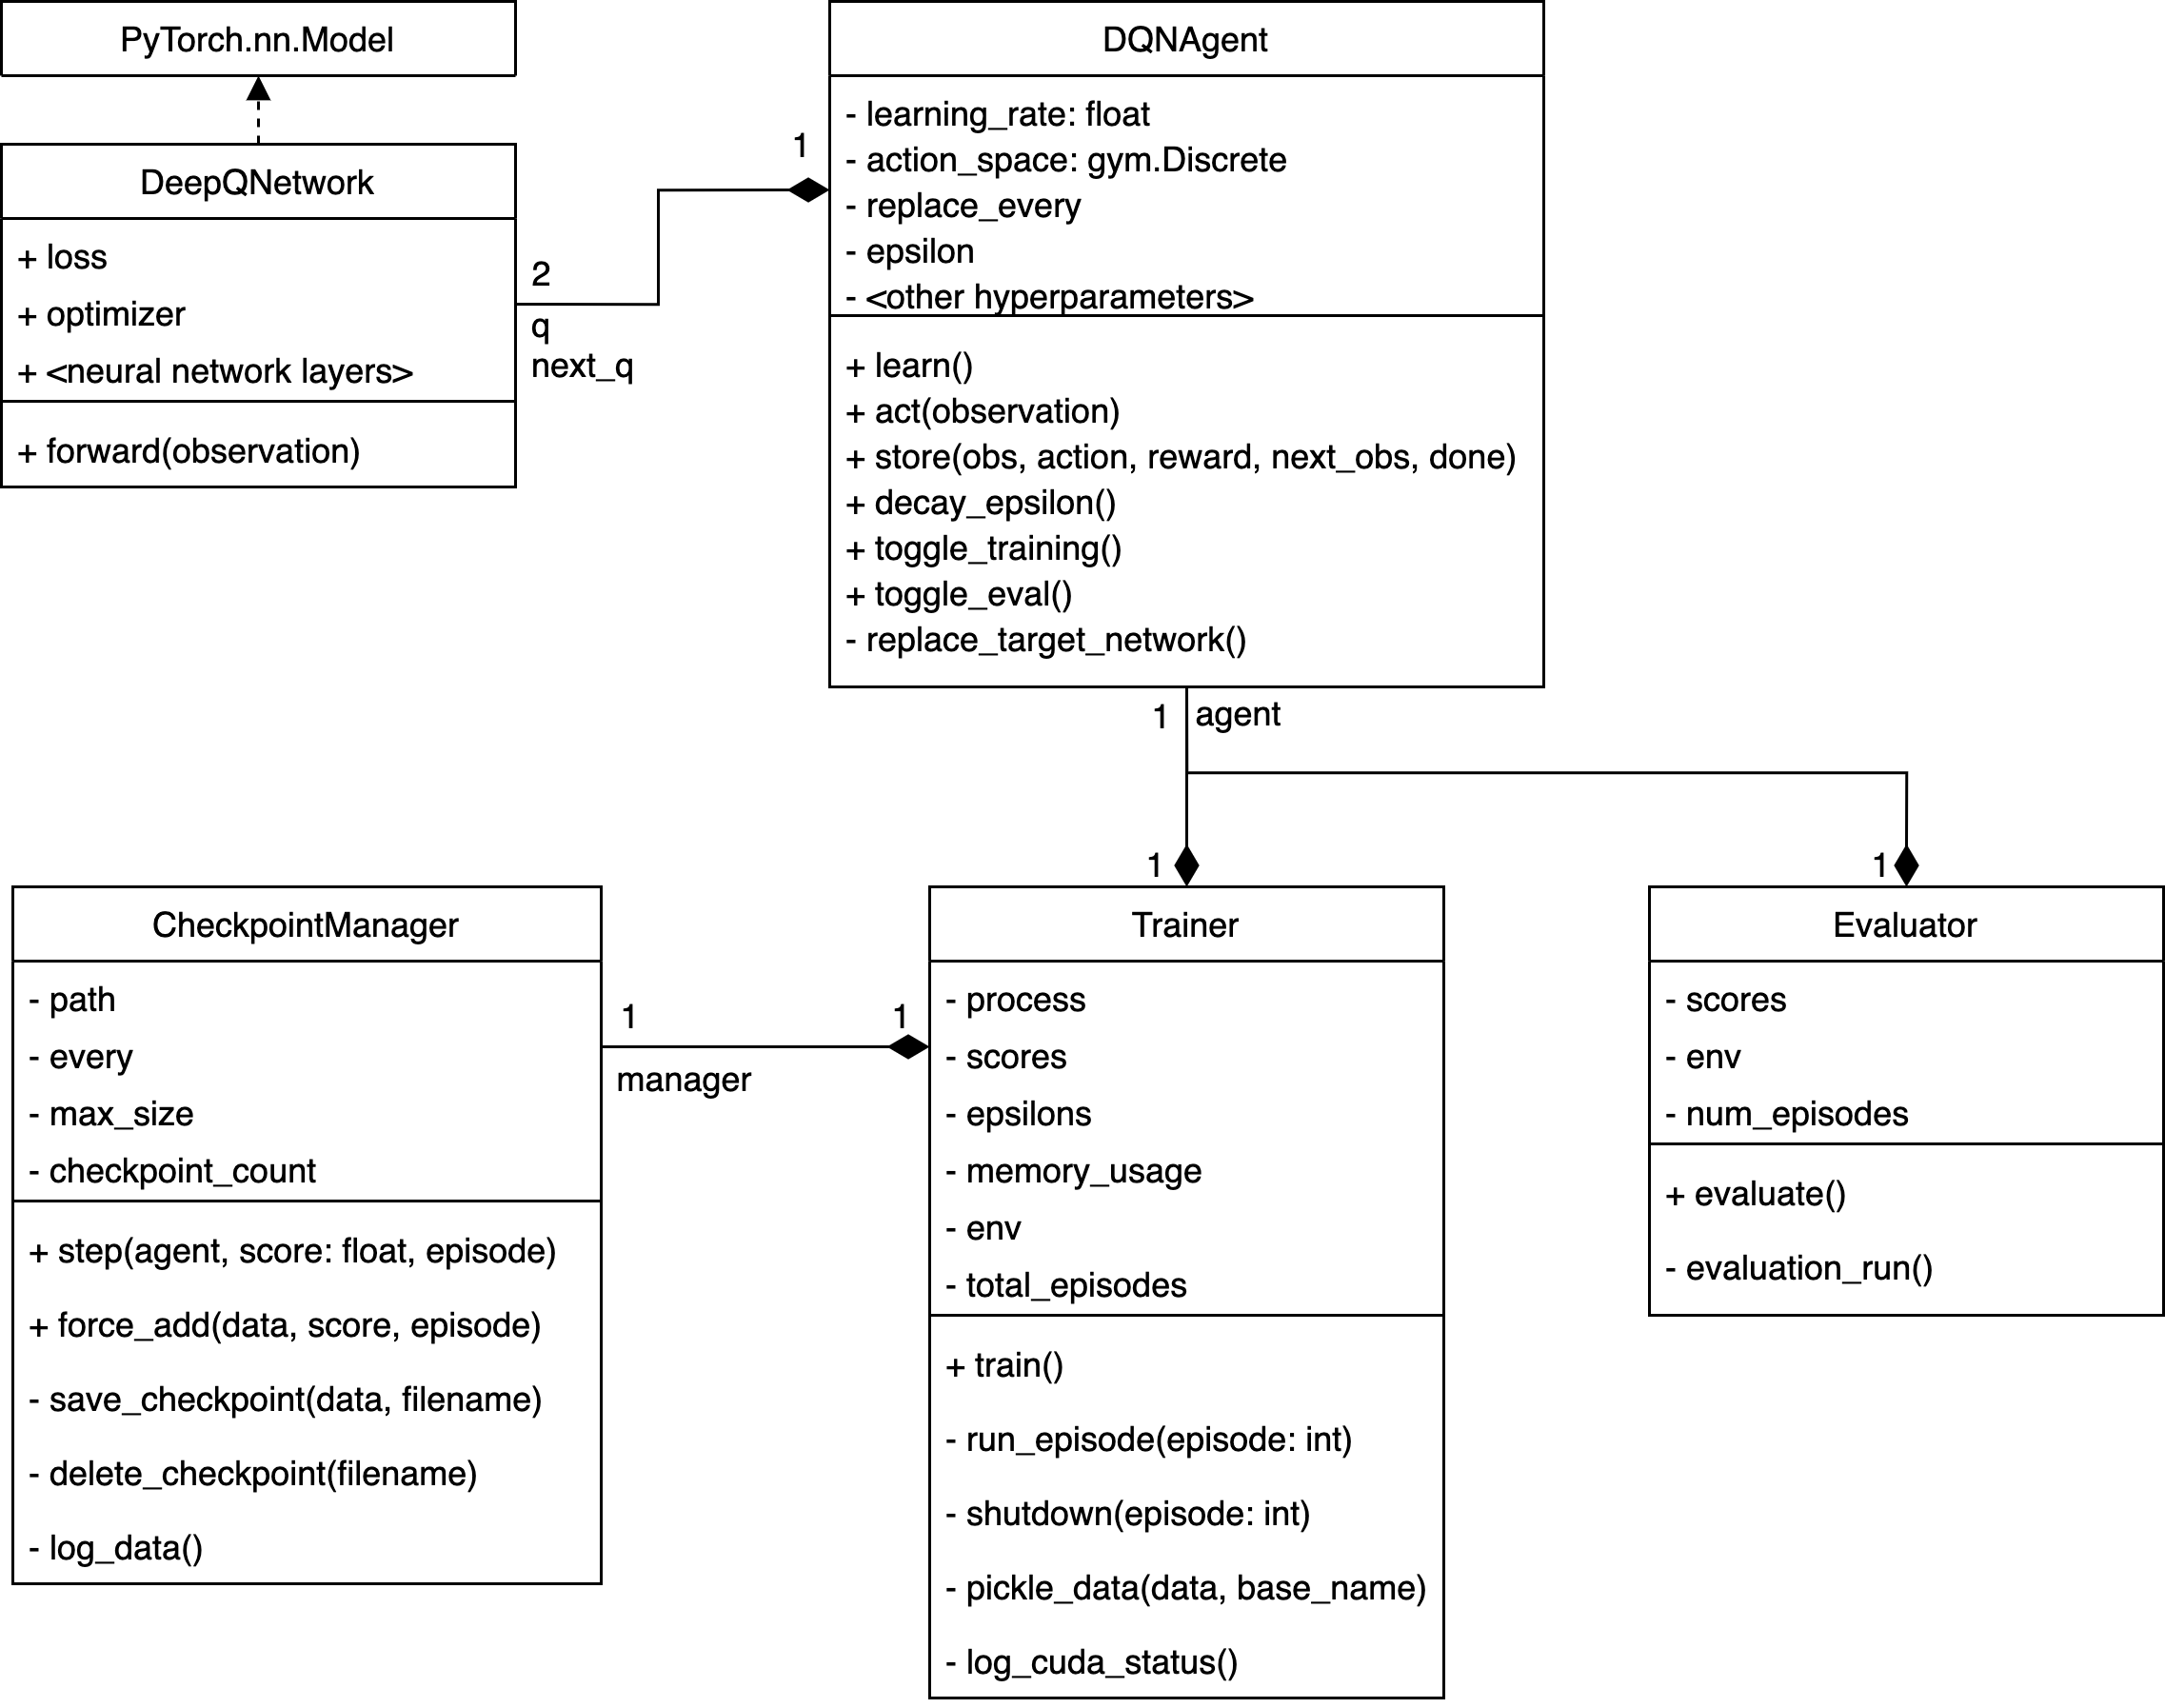
\includegraphics[width=\textwidth]{diagram_central_on_agent.png}
    \caption{A diagram representing how various classes interact with the \texttt{DQNAgent} class.
    The other agent classes follow the same blueprint.
    }
    \label{fig:agent-class-diagram}
\end{figure}

We will dissect the \texttt{deepq} package which, besides being a stand-alone implementation of the original DQN algorithm, represents the foundation upon which the other agents build upon.

The \texttt{deepq.Agent} module encapsulates the algorithm described in the DeepMind paper \cite{atari-dqn}.
An agent entity is initialized from a set of hyperparameters loaded from the configuration file in its \verb|__init__| method.

\begin{figure}
    \centering
    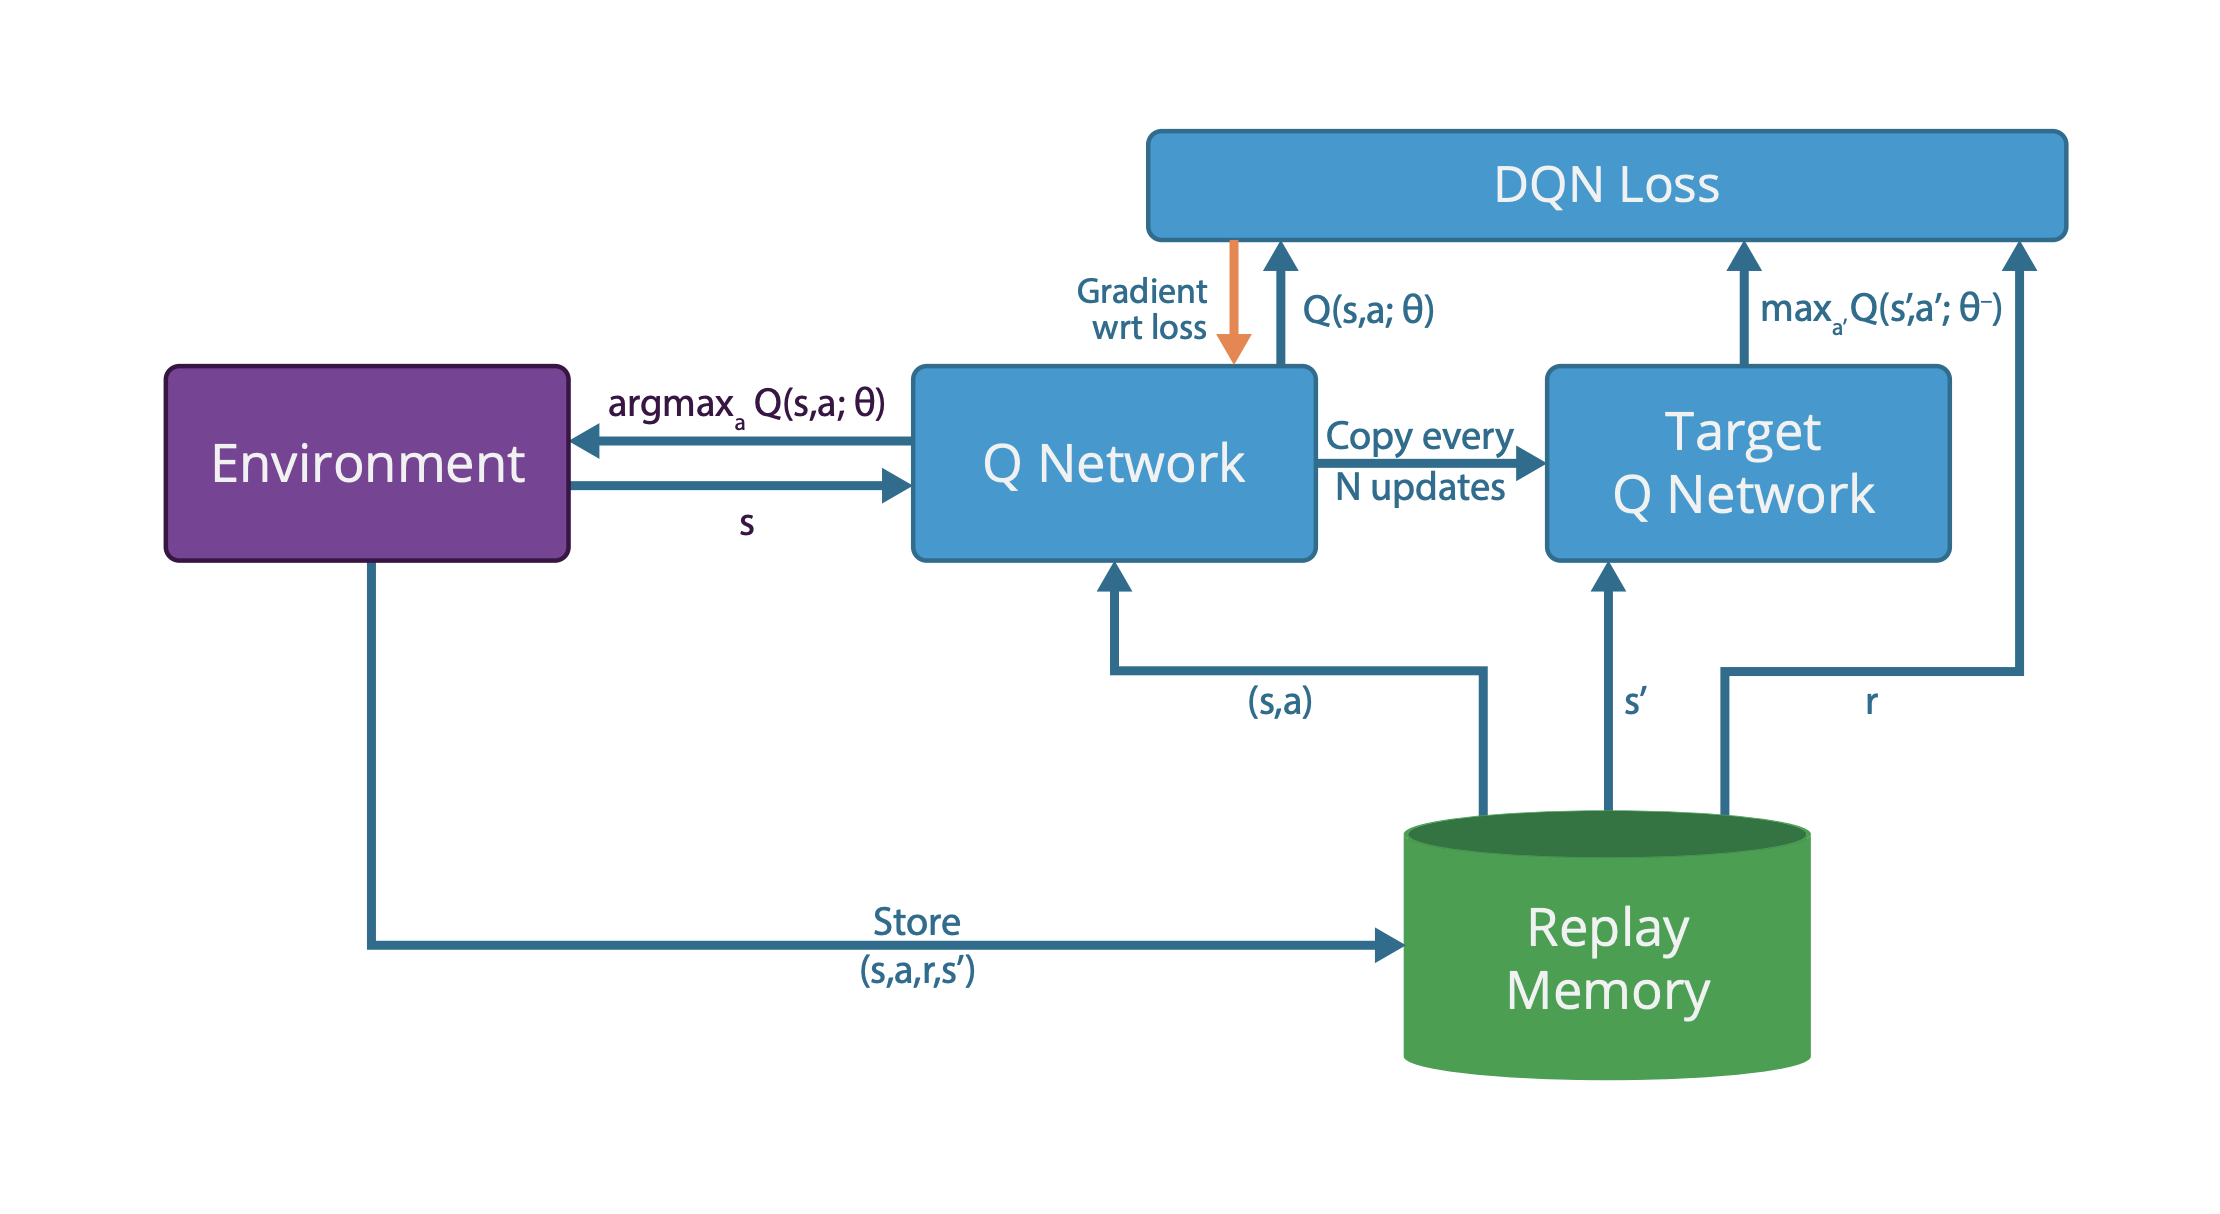
\includegraphics[width=0.9\textwidth]{dqn-architecture.png}
    \caption{High-level architectural view of an agent in classic DQN (Illustration from \cite{mpmdrl}).}
    \label{fig:dqn-architecture}
\end{figure}

The agent is fitted with two networks, which together constitute our model. We will explain in more depth in Subsection \ref{section:model-arch}. The networks are:
\begin{enumerate}
    \item the \textbf{main} Q-network, which provides the basis of action in the environment.
    \item the \textbf{target} Q-network, which estimates the Q-values of the next state.
\end{enumerate}

An agent class’s most central methods are \texttt{act} and \texttt{learn}.

The \texttt{act} method of the \texttt{DQNAgent} entity chooses an action based on an $\varepsilon$-greedy policy.
This essentially means that our agent has a probability $\varepsilon \in [0, 1]$ of choosing a random action.
During the course of our training, $\varepsilon$ will linearly decrease, until a certain point (e.g., we stop at a 5\% chance and keep it there for the rest of our training) -- this is called epsilon decay.

\textbf{Epsilon decay} is implemented by a secondary function in our module, called when a training episode finishes (see \verb|decay_epsilon|).
The process of decaying $\varepsilon$ is crucial to the convergence guarantees of most reinforcement learning algorithms.
It manages proper exploration of the environment.
Without proper control over this aspect, the agent can and will tend to get stuck in local optima.

The \verb|learn| method encapsulates the core of the system and runs one step of mini-batch gradient descent, as explained in Section \ref{section:dqn}.
The steps of the algorithm are broken down below.

Firstly, a mini-batch of transitions is sampled uniformly from our \textbf{replay memory}.
A transition represents a unit of agent experience and has the form $(s, a, r, s')$, where $a$ is an action in the action space, $r \in \mathbb{R}$ is the reward signal, $s$ is an observation (or state) of our agent and $s'$ is its successor state (observed after taking action $a$).

The Q-values are computed by a forward pass through our main network, for all states $s$ in our mini-batch, obtaining the main Q-value matrix.
This process can be accelerated, as the implementation is capable of leveraging GPU processing.
However, we are interested only in the actions $a$ which were taken during the actual play-through of our agent.
We reduce this matrix to a row vector, by only selecting the relevant action $a$ for every set of Q-values.

What in the original paper is denoted as $y_i$ will be computed by the agent in vector form by computing the mean-squared error function of the two vectors.
Using the computed loss, we take a step of mini-batch gradient descent.
Our optimizer is \verb|RMSProp|, as in the original work \cite{atari-dqn}.

Figure \ref{fig:dqn-architecture} provides a high-level recap, using a graphical depiction of how the different components interact during the learning step of the agent.

% \clearpage

\subsubsection{Model Architecture and the \texttt{DeepQNetwork} Class} \label{section:model-arch}

% Add a figure generated with https://github.com/ashishpatel26/Tools-to-Design-or-Visualize-Architecture-of-Neural-Network

Our model consists of two networks, the \textbf{main} and \textbf{target} deep Q-networks.
They are convolutional neural networks, sharing the same architecture.
A deep Q-network is composed of three layers: the first ConvNet layer applies a $8 \times 8$ filter with a stride of 4, the second ConvNet layer applies a $4 \times 4$ filter with a stride of 2, while the final layer is a fully-connected layer with 256 rectifier units \cite{atari-dqn}.
Both convolutional layers are followed by a rectifier nonliniarity.

The \textbf{input} to either network is a stack of $k$ frames, denoted conceptually as $s$ (or $s'$ in the case of the successor state, fed into the target network).
Stacking multiple frames captures the motion aspect of the game environment, which is essential for decision-making.
To reduce the storage space taken by the state representation, any frame captured from the emulator is transformed through gray-scaling, then cropped, to produce an 84 $\times$ 84 grayscale image \cite{atari-dqn}.
This transformation function is implemented as a wrapper around the emulator, in the \texttt{wrappers} package.

The \textbf{output} is a distribution over actions in the finite action space of the environment.
In the case of Pac-Man, the action space consists of four directions.
The available actions are specified by the Gym environment.
Other environments may provide actions for firing a weapon or activating an item.

The above network architecture is implemented in \texttt{deepq.DeepQNetwork} as an extension to PyTorch’s \texttt{nn.Model}.
\texttt{nn.Model} is an abstract class describing a node in a PyTorch computation graph, any extension of which needs to implement the \texttt{forward} and \texttt{backward} methods.
In the case of a neural network, they correspond to the forward pass and the backpropagation step respectively.

\subsection{The \texttt{replay\_memory} Package} \label{section:replay-memory-implementation}

% \begin{figure}[ht]
%     \centering
%     \begin{subfigure}[b]{0.5\textwidth}
%         \centering
%         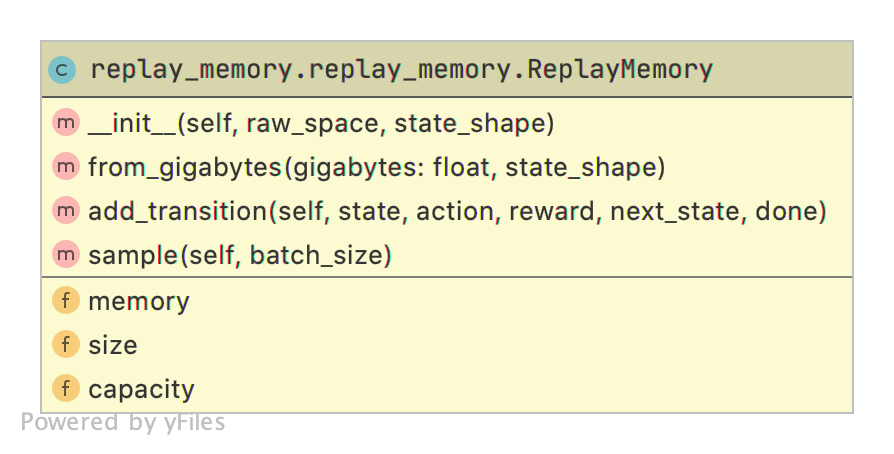
\includegraphics[width=0.5\textwidth]{app-replay-memory-class.png}
%         \caption{Class diagram of \texttt{ReplayMemory}.}
%         \label{fig:rm-diagram}
%     \end{subfigure}%
%     \hfill
%     \begin{subfigure}[b]{0.5\textwidth}
%         \centering
%         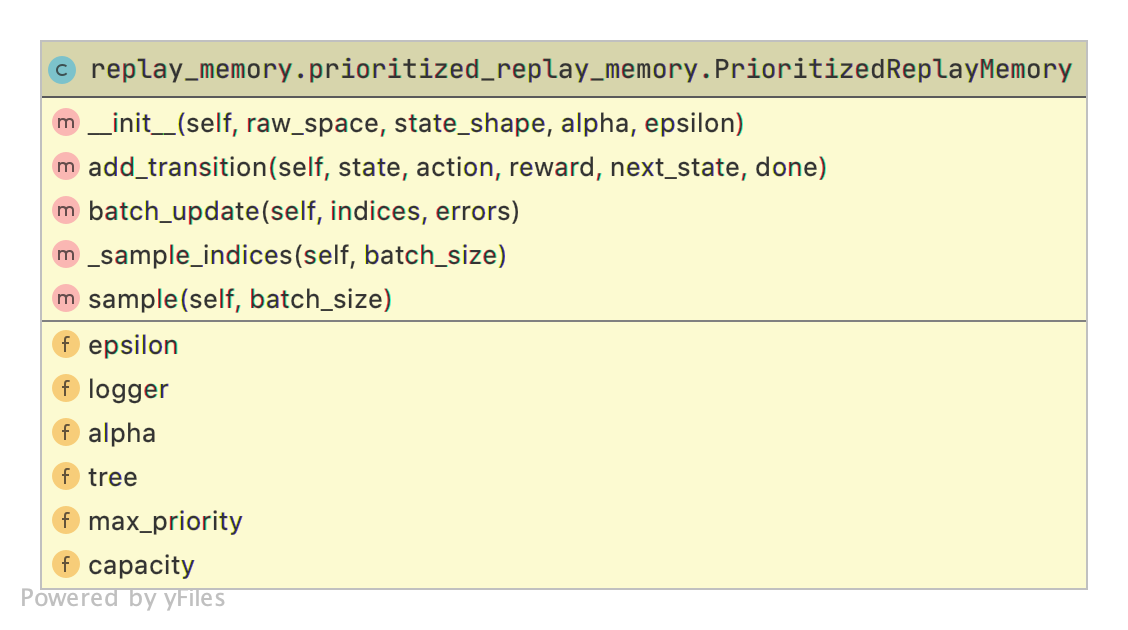
\includegraphics[width=0.5\textwidth]{app-prioritized-replay-memory-class.png}
%         \caption{\texttt{PrioritizedReplayMemory}}
%         \label{fig:prm-diagram}
%     \end{subfigure}
% \end{figure}
\begin{figure}[ht]
    \centering
    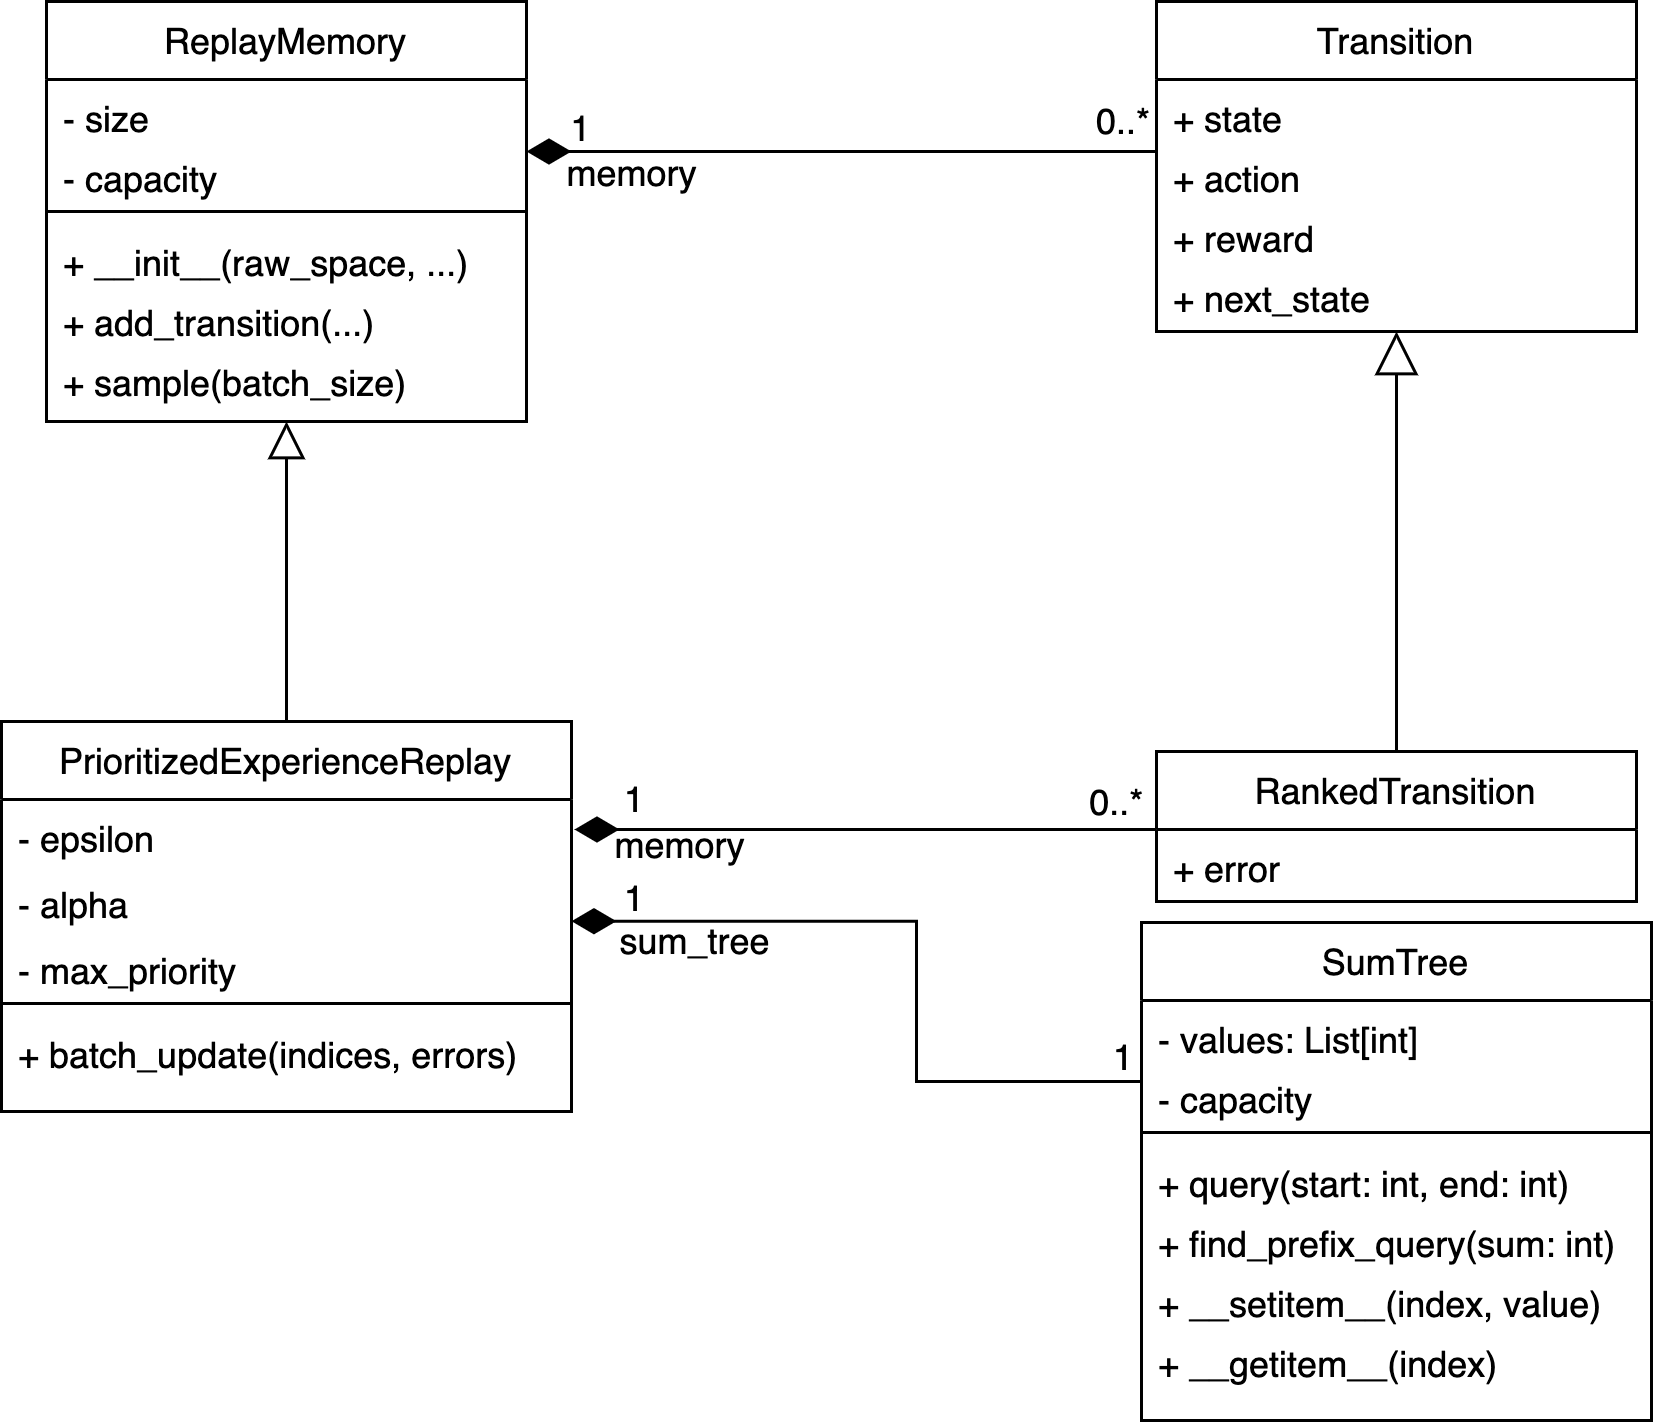
\includegraphics[width=\textwidth]{diagram_central_on_replay_memory.png}
    \caption{Diagram representing the \texttt{replay\_memory} classes and the relations among them.
    \texttt{SumTree} is also shown in this diagram due to its relevance to the functioning of the replay mechanism.}
\end{figure}

The project provides two implementations for the agent’s replay memory.

\texttt{ReplayMemory} provides a simple buffer from which we can sample experiences uniformly at random. This is used in DQN and in double Q-learning as well, as it does not impact the advantages of double learning.

\texttt{PrioritizedReplayMemory} is a more complex mechanism which memorizes the TD-errors of transitions and computes some priorities at every learning step, according to the algorithm in Section \ref{section:per}.
The prioritized sampling operation does not use a uniform distribution.
Instead, we use a sum tree to select transitions according to the error-based probability distribution.

Both implementations are able to deduce their maximum capacity from the total amount of memory (in gigabytes) given in the configuration file.
This mechanism is useful for remote execution on cloud instances, where as the amount of RAM available on the machine is pre-determined. We can specify a fixed chunk of memory to be allocated to the training process, to use as much of the available resources as possible.

\clearpage

\section{Technologies} \label{section:technologies}
Our framework leverages the stability of several battle-tested machine learning libraries.
Our choice of tools allows us to focus on the quality and performance of our implementation.
Our stack supports both CPU and GPU processing and allows quick prototyping, which was essential in the early stages of the project.
Below we present the most important libraries we use and mention their role in our project.
% possible extensions: Google Cloud Compute, TensorBoard, Anaconda, matplotlib

\subsection*{PyTorch}
\textbf{PyTorch} is an open-source machine learning library based on the Torch library.
It was created with a focus on the Python language \cite{pytorch-book} and thus has a strong interface for Python, although a C++ interface is also provided.
PyTorch has been built for speed and provides GPU-accelerated tensor support as well as a strong neural network package -- \verb|torch.nn|.
A distinguishable mechanic of this framework is its auto-differentiation implementation (called \texttt{autograd}) which allows building dynamic computation graphs, making the framework flexible and suitable for quickly prototyping machine learning models.
PyTorch is used in our framework to build the convolutional networks and to perform tensor computations, an integral part of our algorithm implementations.

\subsection*{NumPy}
NumPy is a scientific computing package for Python, supporting linear algebra, and featuring a complex random number library and versatile data structures for vectorized computation.
We use NumPy \verb|ndarray|s as a CPU-only equivalent to PyTorch's tensors, in areas of our program which do not need to support both modes of computation.
For example, the replay memory's buffer is exclusively held in main memory and thus does not require tensors, but we do perform vectorized operations and operations involving randomization.
Besides its speed (NumPy's core functionality is written in C), another important benefit is its comprehensive documentation.

\subsection*{OpenAI Gym}
In order to test our agent implementations, we rely on an excellent solution developed by the OpenAI team.
\textbf{OpenAI Gym} \cite{openai-gym} provides ready-made reinforcement learning environments, as well as flexible tools with which programmers can create their own.
We use OpenAI's supplied Atari environments, which provide interfaces to keep track of in-game score, lives, health or other indicators.
Those variables, primarily the score, serve as factors in the reward computation.

\subsection*{Jupyter Notebook}
Jupyter Notebook is a web-based environment for creating interactive ``notebooks'' -- documents which interleave Python code with Markdown notes, \texttt{matplotlib} plots and other objects.
They are a great tool for quickly prototyping models and documenting one's solution to a problem and are in widespread use in the Python data science community.
Juypter Notebook is only one project among many released by Project Jupyter as open-source software.
We extensively used notebooks for protyping during the early phase of the framework.
We incorporate a separate directory for special notebooks for studying algorithm performance, to plot agent performance and to compare different training runs.

\section{User Manual} \label{section:user-manual}
This section presents the basics of operating our framework to use one of our existing agents in the library to run a training job and collect its data.
Below we list commands for training, evaluation and deployment and we explain flags and configuration variables.

\subsection*{Training}
Training can be initialized locally, on the user's computer, or remotely, in a cloud environment.
The starting script \verb|train.py| initializes the \verb|Trainer|, changes its mode of operation based on the relevant flags and loads the configuration file.
\begin{verbatim}
python train.py -c <configuration-file> <options>
\end{verbatim}

This is an example of a \verb|YAML| configuration file, written for the DQN algorithm:
\begin{verbatim}
training:
  name: dqn
  ...
model:
  learning_rate: 1e-4
  gamma: 0.99
  ...
checkpoints:
  path: ../data/checkpoints/
  max_size: 5
  every: 500
logs:
  path: ../data/logs/
monitor:
  path: ../data/monitor/
evaluation:
  num_episodes: 200
  ...
\end{verbatim}

The \verb|training| node contains general information about the training job, including a label to track it when comparing multiple results.

The \verb|model| node contains hyperparameters required by a particular algorithm to run.
A lot of the parameters are common among the various implementations (for example, \verb|learning_rate| is a general parameter of the neural network).

The \verb|checkpoints| settings group controls the checkpoint manager, as discussed in its relevant subsection in the \emph{Implementation} section.

\verb|monitor| and \verb|evaluation| control the \textbf{evalutation}. Those are not relevant to the training per se, but sometimes we want to associate the evaluation settings to the algorithm itself, so we can put them into the same file, instead of having two separate configurations (although using separate configurations between traning and evaluation is possible).

Before the launch of the training job, the user can specify the desired algorithm using two special flags.
\verb|--per| trains the agent using prioritized experience replay.
\verb|--doubledqn| train the agent using double Q-learning.
Combining these flags in whichever order will enable both approaches simultaniously by loading and training the \verb|DoublePERAgent|.

\subsection*{Evaluation}
For evaluation, we similarly run:
\begin{verbatim}
    python play.py -c <configuration-file> <options>
\end{verbatim}

The evaluation environment is designed to test an agent in a more stable environment, with no randomization.
This running mode has the addition of outputing \textbf{video captures} of the emulator in a dedicated \verb|monitor| directory (as specified by the \verb|monitor.path| setting in the configuration), so that we can study an agent's behaviour by directly observing any strategies it might have developed or any areas in which it have failed to develop one.

\subsection*{Utility Scripts}
The \verb|data| directory stores the data associated to the training job, including logs, scores and checkpoints.
At the end of training, this directory is compressed into a \verb|results| file (using the \verb|gzip| standard) so the data directory itself is redundant and needs to be cleaned.
For this purpose, we provide a \verb|cleanup.sh| Bash script, for $*$nix systems, which removes the training files and re-initializes the required directory structure.

Additionally, we might want to make modifications to the implementation and want to keep the Python codebase compliant to PEP norms.
For this purpose we use the \verb|black| code formatter and the \verb|docformatter| utility for docstrings.
We provide a \verb|format.py| Python script, which combines those two and runs them recursively over every directory in our codebase, in order to keep everything tidy and uniformly stylized.

% might add TensorBoard usage


\chapter{Results and Evaluations}
This chapter introduces our methodology, presents our experiment setup and results, and compares them to the expectations set by existing benchmarks.
First of all, we introduce and justify the methods we use to evaluate agent performance in the Pac-Man environment.
We then show the results obtained using the chosen technique and analyze them, using the tools provided in our framework.
We comment on those results and compare them to what other similar studies have shown.

\section*{Evaluation in Reinforcement Learning}
\textbf{Evaluation} is a fundamental part of any machine learning project and reinforcement learning is not an exception to this rule.
The goal of evaluation in RL is compatible with the goal of its encompassing field and is analogous to that of supervised learning, in the sense that both are concerned with measuring how well a model \emph{generalizes}.

The aim of evaluation in RL is to measure the extent to which the acquired behaviour of the agent generalizes to the class of environment it learned in.
In other words, researchers try to certify if the agent learns meaningful \emph{skills} -- patterns in behaviour which are general enough to solve the problems they are developed to solve, even if presented from a new perspective.

In a similar manner, in supervised learning, models are evaluated based on their ability to accurately predict, estimate or classify previously unseen data -- their generalization ability.
A key difference between RL and its supervised counterpart is the latter's clearer methodology of dividing the dataset.
Experiments in supervised learning can and must split their data into specific subsets -- one for training and one for evaluation. In the RL setting, this separation is seldom possible.

Attempts to correct this overlap between training and evaluation in experimental RL is an active area of research.
One compelling paper concerning itself with this problem, published by OpenAI researchers, proposes building \emph{procedural generation} into environments \cite{procgen-paper}.

\section*{Setup and Methodology}
The evaluation \textbf{methodology} we chose for this thesis was used before across numerous RL studies, including in DeepMind's DQN and Double DQN works \cite{atari-dqn,ddqn-paper} and has been originally proposed in the Atari Learning Environment (ALE) paper \cite{ale-paper}, which was specifically developed to analyze agent perfromance in video game environments on the Atari 2600.
We follow the above guidelines closely, with a few exceptions.
For example, we will not be including including human performance in our benchmark.

% REFACTOR THIS --------------------------------------------------------------
% To prevent overfitting, the environment has \textbf{added stochasticity}.
% A significant portion of video game environments are deterministic by nature, including Pac-Man.
% If the agent were to replay the same sequence of moves over multiple gameplays, the environment would respond in the exact same way.
% The problem is that an ``imposter’’ agent could overfit and memorize the level over time, resulting in an agent that can solve the level reasonably efficiently, but which fails if we tweak even fine details.
% This is prevented by the stochasticity of the environment and the stochasticity of its own model.
% In order to ensure that no two training runs are the same from an environmental stand-point, the agent’s choice is replayed in the environment.
% This can be a fixed or a random number of times, which we denote $k$.
% Some task environments choose a $k$ in $[1, 3]$.
% We use the fixed variant\footnotemark{} of this technique, which has been proposed and used by the DeepMind team in the original DQN study \cite{atari-dqn}.
% \footnotetext{DQN uses $k = 4$ for most games, except for Space Invaders which requires $k = 3$ because of an overlap with the period at which the projectiles blink \cite{atari-dqn}.}

Additionally, we use \textbf{epsilon annealing} for the $\varepsilon$-greedy policies, another technique in the DQN standard.
The approach consists of linearly decreasing epsilon from $1$ to a predetermined lower bound, usually $10\%$ or $5\%$, to ensure non-zero exploration probability over the entire training run.
The role of this is to ensure that the agent does not get stuck in a local optimum, as well as to prevent overfitting to the environment.
If we allow the exploration coefficient to go all the way to zero, we risk having an agent learn a pattern that is inefficient or even counterproductive and would have no way of stopping it short of restarting the training run.

Our experiment setup starts from well-established standards in order to find ways to tweak them.
The implementation we use for our task environment is \texttt{MsPacman-v4}, provided by OpenAI within the \texttt{gym} package.
The base name of the game is \texttt{MsPacman}, designating the Atari 2600 version of Pac-Man.
The package offers multiple variables which control stochasticity of the environment.
An environment labeled \texttt{Deterministic} will have a fixed frameskip, set to $k = 4$ in our case.
The label \texttt{v4} indicates that the agent action is not repeated (besides the frame-skipping aspect), in contrast to \texttt{v0} which specifies a 25\% chance the previous action is repeated.

Our choice of hyperparameters is illustrated in Table \ref{tab:our-hyperparameters}.

\begin{table}
    \centering
        \begin{tabular}{ll}
        Variable                           & Value   \\
        learning rate $\alpha$             & 1e-4    \\
        discount factor $\gamma$           & 0.99    \\
        initial $\varepsilon$              & 1       \\
        terminal $\varepsilon$             & 0.05    \\
        $\varepsilon$ decay                & 8.62e-5 \\
        batch size                         & 32      \\
        swap frequency (number of steps)   & 1000    \\
        PER $\alpha$                       & 0.6     \\
        PER $\epsilon$                     & 0.01
        \end{tabular}%
    \caption{Hyperparameters used to train our agent models.}
    \label{tab:our-hyperparameters}
    \end{table}

% gym
% hyperparameters

\section*{Results}
% plot some graphs
% write the conclusion
% read Roman Ring's thesis again

\chapter{Architecture}
\input{chapters/architecture}

\chapter{Conclustion and Future Work}
In this thesis, we introduced the fundamentals of \emph{reinforcement learning} -- a field of machine learning concerned with developing systems which learn based on interaction with the environment.
What distinguishes RL from other methods is the concept of reward signal, which provides feedback on whether the system behaves in a desirable way, from the perspectives of the goal of a task.

The transfer of knowledge from deep learning to the classical methods in RL is revolutionizing the field.
In the second part of Chapter \ref{chapter:background}, we presented some of the techniques that emerged to build more performant intelligent agents, leveraging the strength and robustness of neural networks, and especially of the ConvNet architecture.

In order to demonstrate the principles of deep RL in action, we have implemented a light framework, featuring a collection of algorithms in deep Q-learning, originally described in \cite{atari-dqn}, and its successors in the DQN family.
We benchmark and analyze the performance of our selected approaches on our task environment of choice -- Pac-Man. Solving Pac-Man is an interesting task and features some open challenges, as mentioned in Section \ref{section:modelling-the-problem}.

The following paragraphs give a summary of the most notable \emph{areas of potential improvement} for this work.

One possible extension to this thesis is hyperparemeter search.
\textbf{Hyperparameter tuning} or \textbf{search} is a problem in machine learning, which consists of tuning the set of hyperparameters to maximize the usefulness of the learning approach \cite{hyperparam-search-paper}.
Most studies have relied on the entire set of 49 Atari games to study the efficiency of their approaches.
In our thesis, however, we solve a more precisely defined task and could have benefited from tuning hyperparameters to some extent.
There is a strong probability that the set of hyperparameters which worked the best on Pong or Enduro does not work as well in Pac-Man.
However, one problem with auto-tuning is a practical problem, in that applying it to a relatively large problem such as ours requires a large amount of continuously-available compute resources.
On the basis of these large computation costs, we have decided that it would be cost ineffective.

Another such extension point is including policy-based and actor-critic methods into the benchmark.
In our background section, we touch on the subject of policy-based methods and their particular advantages.
The problem with policy-based RL is the novelty and increased complexity of the algorithms, over the more well-established techniques.
In other words, the state-of-the-art is not accessible to entry-level enthusiasts and would require far more work to implement from scratch, test and deploy.

To sum up, we have seen that autonomous RL agents can learn useful behaviour.
However, the study of autonomously learning RL agents in games has not been without challenges.
As we have seen with DQN and its successors, its greatest weakness remains sample efficiency -- agents need to train for millions of steps before they demonstrate any significant amount of ability.
And even then -- as we pay closer attention to generalization in deep RL -- we find that most Q-learning-based methods only manifest a somewhat limited ability to generalize, outside of very simple strategies (such as Pong, the game with the highest score obtained by DQN \cite{atari-dqn}).

With this in mind, the road ahead looks bright for RL, with a recently released paper from DeepMind – \emph{Agent57} (2020) \cite{agent57-paper}. We note that the latest research trends seem to be using mixed approaches: DQN and policy optimization algorithms, in an attempt to break the barriers set by their predecessors.
\emph{Agent57} has managed to break every record on the Atari benchmark and has obtained scores above the human baseline on 57 games in the set.

\bibliography{references}

\end{document}